% Class for the academic internship paper :
\documentclass[utf8,final]{stageM2R}

\usepackage{graphicx}
\usepackage[T1]{fontenc}
\usepackage{float}
\usepackage[french]{babel}
\usepackage[draft]{commands} % Custom commands, defined in this folder
\setsecnumdepth{subsection}

\supervisors{Noura \textsc{Faraj}\\Christophe \textsc{Fiorio}\\Benjamin \textsc{Charlier}}
\location{LIRMM UM5506 - CNRS, Université de Montpellier}
\title{Gestion, traitement et visualisation d'images médicales à très haute résolution}
\track{IMAGINA}
\date{2 Juillet 2020}
\author{Thibault}
\abstractfr{Ce sujet de stage s'inscrit dans un effort de collaboration internationale entre l'université de Tulane à la Nouvelle Orléans, et l'université de Montpellier dans le cadre d'un projet pour l'aide à la détection et au diagnostic du cancer de la prostate.}

\begin{document}
	\selectlanguage{french}
	\frontmatter \maketitle
	\cleardoublepage
	\settocdepth{subsection} \tableofcontents \mainmatter

	% Chapitre 1 : Introduction
\chapter{Introduction}\label{chapter:01:introduction}
{
	\commentaire{
		\begin{enumerate}
			\item introduction au sujet de stage~\begin{itemize}
				\item présentation de la reconstruction 3D
				\item intérêt dans le médical
				\item transition : présentation de la prostate (à revoir)
			\end{itemize}
			\item introduction à la problématique (coupes histologiques, Gleason, ...)~\begin{itemize}
				\item prostate : beaucoup de cancers
				\item cancer de la prostate : identifier $\rightarrow$ échelle de Gleason
				\item présentation rapide de l'échelle de Gleason
				\item intérêt de la reconstruction 3D : vraie forme des glandes.
				\item (?) intérêt du stage : Tulane ne le fait pas
				\item transition (?)
			\end{itemize}
			\item rapide overview du travail fait~\begin{itemize}
				\item présentation du chargement des images
				\item présentation de la recherche de voisins
				\item présentation de la génération de grille de voxels
			\end{itemize}
		\end{enumerate}
	}\par

	\wip{La reconstruction 3D permet d'obtenir une représentation tridimensionnelle d'un objet ou d'une scène à partir d'un ensemble de primitives, tells que des points, des images ou des sous-ensembles tridimensionnels. Ces représentations tridimensionnelles des objets permettent de mieux percevoir le fonctionnement et l'utilisation implicite d'un objet grâce aux affordances qu'il nous permet d'inférer.\todo{Vraiment nécessaire ? On sait que c'est mieux en 3D, mais trouver meilleure excuse.}}\\

	\wip{Naturellement, une représentation tridimensionnelle et interactive [...]}\\

	\wip{Ce sujet de stage s'inscrit dans un effort de collaboration internationale entre l'université de Tulane à la Nouvelle Orléans, et l'université de Montpellier dans le cadre d'un projet pour l'aide à la détection et au diagnostic du cancer de la prostate. Ainsi, il est nécessaire de préciser certaines choses sur les caractéristiques de cette pathologie.\\Tout d'abord, selon l'IARC, l'Agence Internationale pour la Recherche sur le Cancer de l'Organisation Mondiale de la Santé, le cancer de la prostate était l'un des types de cancers les plus courants tous sexes confondus en 2018\footnote{Voir : \protect{\url{https://gco.iarc.fr/today/home}}}. Cette même année, plus d'un million nouveaux cas de cancers de la prostate furent diagnostiqués dans le monde.}\\

	\wip{Le meilleur pronostic disponible est une échelle histologique, appelée échelle de Gleason. Celle ci attribue un score, appelé score de Gleason, en se basant sur l'observation des formes des glandes dans une coupe du tissu de la prostate d'un patient. Or, étant une échelle se basant sur l'observation de la forme des glandes dans une coupe histologique, donc effectivement bidimensionnelle, d'un objet tridimensionnel, le biais induit par la direction et l'angle de la coupe influera beaucoup le pronostic final donné par un praticien. Ainsi, cette méthode de pronostic pourrait engendrer de faux pronostics, pouvant soit causer des frais médicaux non nécessaires pour un patient sain, mais aussi pouvant laisser le cancer d'un patient se développer librement, sans aucune action prise à son encontre.}\\

	\wip{Dans ce contexte, une reconstruction 3D permettrait d'effectuer un meilleur pronostic en étudiant la forme réelle des glandes. Le but du projet, à long terme, serait de créer une nouvelle procédure de diagnostic du cancer de la prostate, utilisant l'information contenue dans la forme réelle (tridimensionnelle) des glandes.}\\

}
% VIM modeline : do not touch !
% vim: set spell spelllang=fr :

	% Chapitre 02 : Etat de l'art
\chapter{Une approche tridimensionnelle pour le diagnostic du cancer de la prostate}\label{chapter:02:presentation_probleme}
{
	
	% Intro chap2 {{{
	De nos jours, les diagnostics du cancer de la prostate sont effectués en utilisant une échelle histologique 2D appelée échelle de Gleason~\cite{cite_gleason_score}. Cette échelle permet de reconnaître le stade d'avancement de la maladie selon les formes des glandes dans un échantillon de prostate en  comparant une image d'une coupe 2D à une approximation graphique faite par Dr. \textsc{Gleason} (voir \ref{section:gleason_scale}). L'utilisation de cette échelle %ne permet pas un diagnostic précis 
	entraîne une variabilité de diagnostic importante car dépendante de l'orientation de la coupe 2D. C'est pour cela que des méthodes de diagnostics utilisant de l'information tridimensionnelle sont en cours de développement.
	%L'équipe de bio-ingénierie de l'université de Tulane a développé une méthode d'imagerie permettant de reconstruire un échantillon en trois dimensions. Appliqué au diagnostic du cancer de la prostate, nous pourrons analyser la morphologie tridimensionnelle des glandes, encore inconnue. L'objectif est de mettre en place une méthode de diagnostic pouvant accompagner les méthodes actuelles telles que l'échelle de Gleason, pour enrichir les méthodes de diagnostic du cancer de la prostate. Notre tâche est de reconstruire cet échantillon rapidement et de manière fiable, à partir des images extraites de leur processus d'acquisition.
	% }}}
	
	Cette section présente la technique d'imagerie 3D développée à l'université de Tulane ainsi que le jeu de donnée résultant que nous avons à disposition.
	
	% Section Gleason {{{
	\section{L'\'echelle de Gleason}\label{section:gleason_scale}
	{
        % IMG : Echelle de Gleason {{{
		\begin{figure}[!h]
		    \centering
		    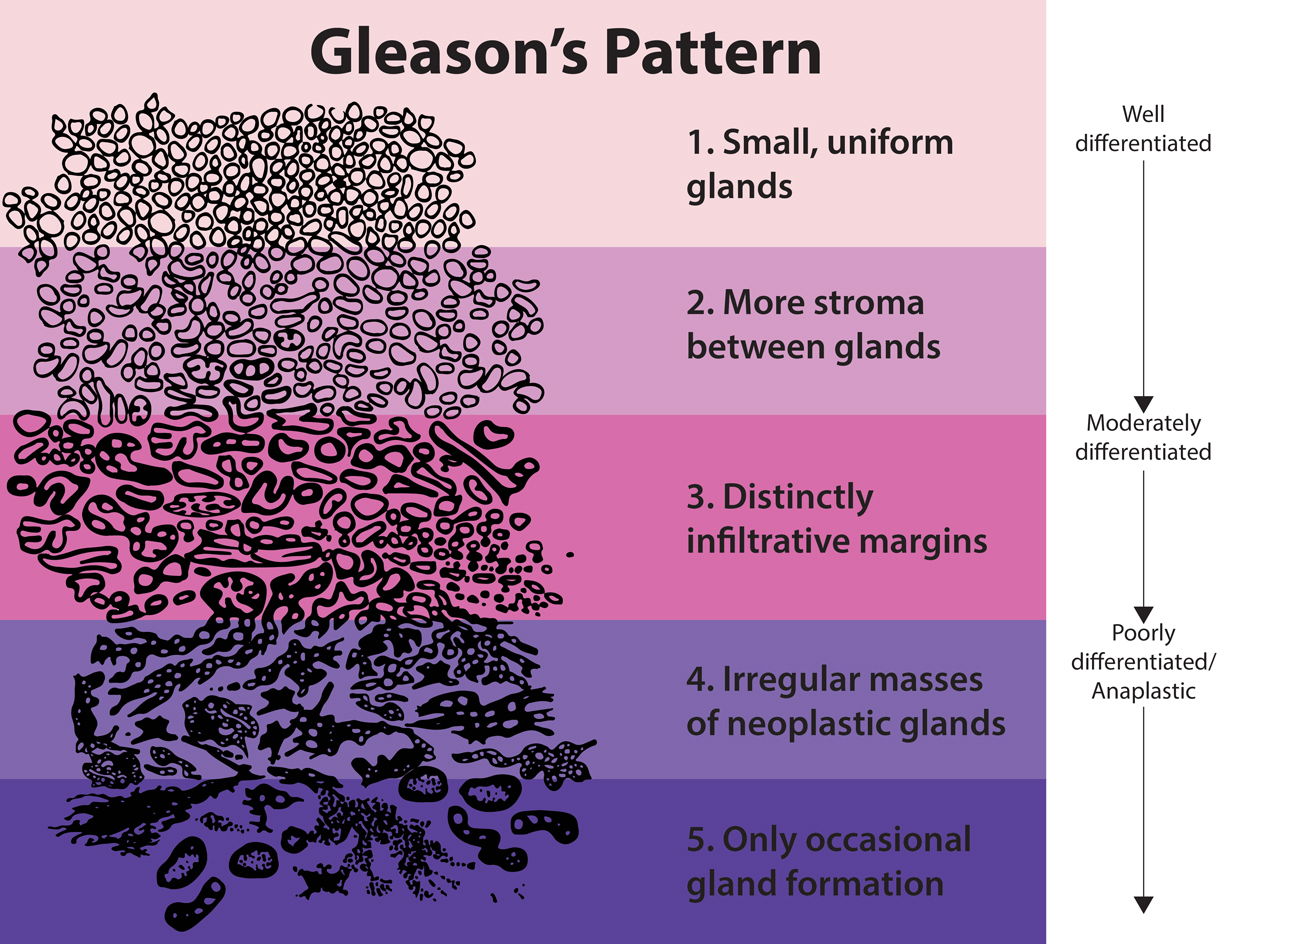
\includegraphics[width=.7\linewidth]{img/gleason_score.jpg}
		    \captionsetup{width=.8\linewidth}
		    \caption{L'échelle de Gleason, représentée schématiquement}
		    \label{img:gleason_scale}
		\end{figure}
		% }}}

		L'échelle de Gleason~\cite{cite_gleason_score} est une échelle pronostique qui se base sur l'observation de la forme des glandes d'une prostate afin d'évaluer la possibilité de présence d'un cancer chez un patient. Inventée par Donald \textsc{Gleason} entre 1960 et 1970, elle permet une évaluation de la présence et de l'avancement du développement d'un cancer de la prostate chez un individu. Cette échelle permet d'attribuer un score de 1 à 5 en fonction de la forme des glandes dans une coupe histologique de la prostate (voir figure \ref{img:gleason_scale}) par rapport à un diagramme fait par Dr.\textsc{Gleason} lors de ses recherches.

		Étant donné que cette échelle se base sur l'observation de coupes histologiques de la prostate, la direction des coupes, l'angle de celles-ci, ainsi que leur orientation influent beaucoup sur la forme observée des glandes de la prostate et donc sur le pronostic final donné par un médecin après observation (voir figure \ref{img:gleason_bias}).

		Afin de pallier cette incertitude, une des méthodes proposée par nos collaborateurs à la Nouvelle-Orléans consiste à analyser la morphologie tridimensionnelle des glandes. En effet, grâce à la méthode de microscopie \textit{di-SPIM}, nous pouvons obtenir une pile de coupes d'un échantillon permettant de construire une grille volumique le représentant. L'élaboration d'une méthode utilisant la morphologie tridimensionnelle des glandes pourrait permettre d'enrichir les connaissances liées à la détection du cancer de la prostate afin de détecter la pathologie plus rapidement, permettant de mieux la traiter par la suite. Une telle méthode viendrait étoffer les méthodes de diagnostic actuelles de détection du cancer de la prostate.
	}
	% }}}

	% Section microscopie {{{
	\section{Microscopie LSFM \& SPIM}\label{section:microscopy}
	{
		La microscopie \textit{LSFM}~\cite{cite_lsfm_explication_girard}, pour \textit{Light-Sheet Fluorescence Microscopy} ou microscopie par fluorescence à feuille de lumière en français est une méthode d'acquisition d'images. Elle consiste à illuminer une tranche de l'échantillon à analyser une fois rendu transparent perpendiculairement à l'axe du système de détection du microscope. La fluorescence de l'échantillon est alors un indicateur du tissu analysé. Plusieurs variations de la méthode existent, notamment une alternative appelée \textit{SPIM}~\cite{cite_spim_explication_original} : \textit{Single Plane Illumination Microscopy}, ou microscopie par éclairage planaire sélectif en français. Cette méthode permet de faire des acquisitions d'échantillons par pile de coupes rapidement, et permettant par la suite une reconstruction 3D de ceux-ci.

        % IMG : SPIM processus capture {{{
		\begin{figure}[!h]
			\centering
			
\includegraphics[width=0.5\linewidth]{./img/lsm_methode_01.jpg}
			\captionsetup{width=.8\linewidth}
			\caption{Processus d'acquisition par \textit{SPIM} : un rayon lumineux (en bleu) est envoyé dans l'échantillon, et la fluorescence de celui-ci est détectée par le dispositif de détection dans sa zone focale (en jaune)}
			\label{img:lsm_01_how_it_works}
		\end{figure}
		% }}}

		Tout comme la méthode \textit{LSFM}, la méthode \textit{SPIM} utilise la fluorescence d'un échantillon afin de l'analyser. Toutefois, la méthode SPIM utilise un éclairage latéral, ce qui permet de rendre les dispositifs d'éclairage et d'acquisition complètement indépendants.

		Les acquisitions sont faites grâce à des émissions de lumière dans l'échantillon à analyser. Ceci entraîne un problème : l'image d'un point de l'échantillon dans l'acquisition s'étale le long de l'axe d'émission. Cela cause une anisotropie\definition{L'anisotropie entraîne des propriétés différentes selon des directions différentes} de la fonction d'étalement de point\footnote{Réponse impulsionnelle d'un système d'imagerie à une source ponctuelle.} du capteur sur son axe dans l'acquisition par coupe d'un échantillon avec la méthode \textit{SPIM} (figure \ref{img:spim_01_point_spread_function}). Pour pallier ce problème, il existe une alternative à la méthode \textit{SPIM}, appelée \textit{di-SPIM}, pour \textit{dual inverted SPIM}. Cette variation consiste à utiliser en tandem deux dispositifs \textit{SPIM} afin d'éliminer l'anisotropie qui existe avec les méthodes de \textit{SPIM} traditionnelles. Un dispositif \textit{di-SPIM} est illustré en figure \ref{img:lsm_02_device}.

        % IMG : Photo microscope {{{
		\begin{figure}[!h]
			\centering
			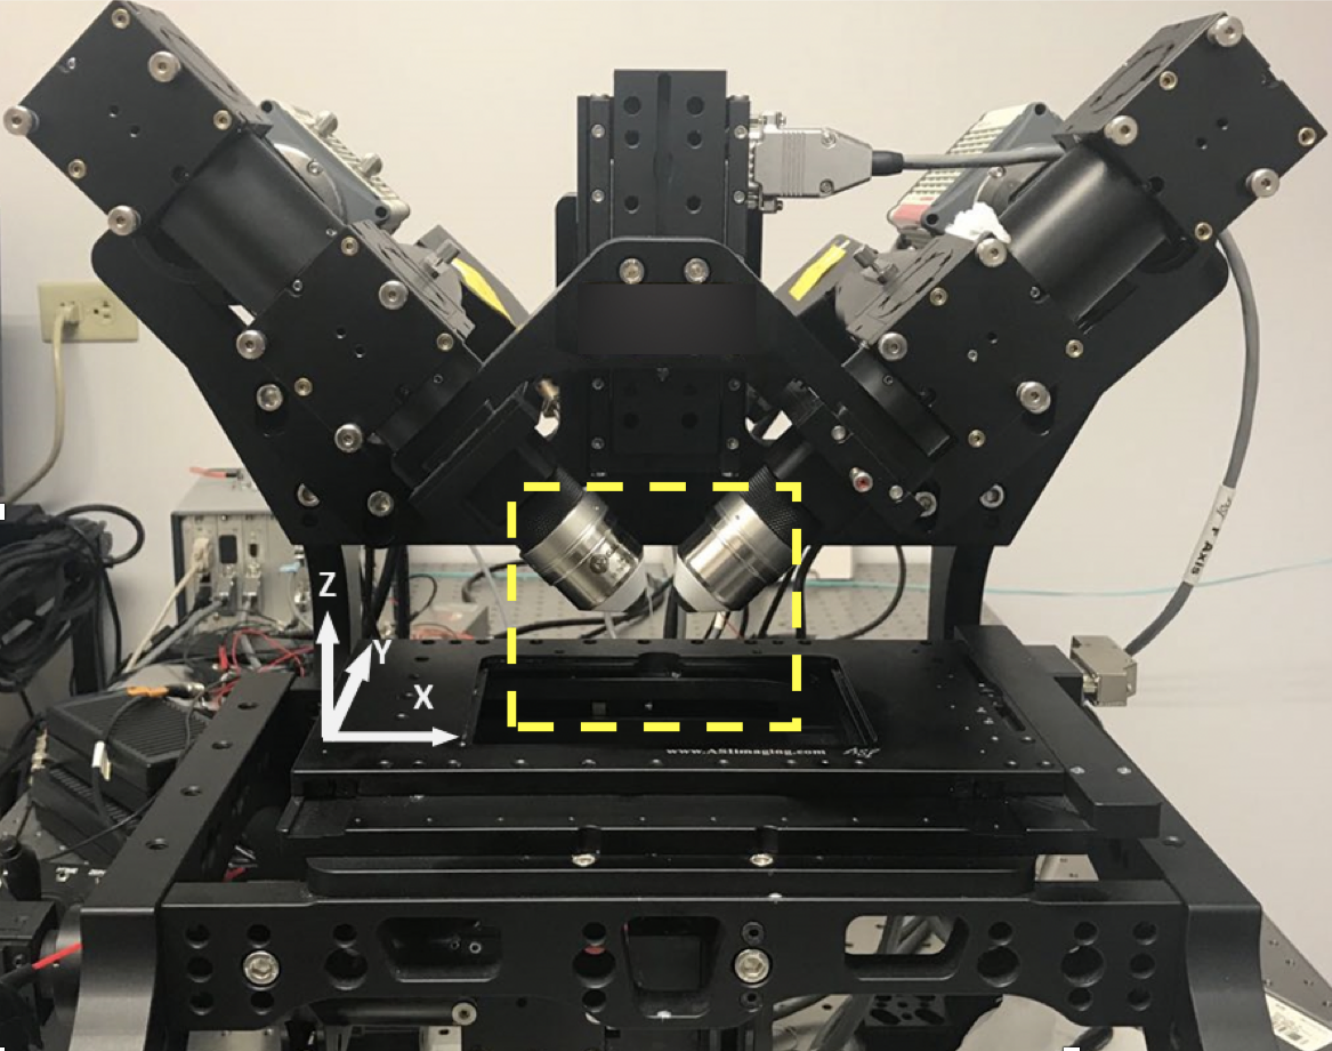
\includegraphics[width=0.5\linewidth]{./img/lsm_device_02.png}
			\captionsetup{width=.8\linewidth}
			\caption{Le microscope \textit{diSPIM} conçu par les chercheurs de la Nouvelle-Orléans permettant une acquisition tridimensionnelle d'un échantillon de manière fiable et rapide.}
			\label{img:lsm_02_device}
		\end{figure}
		% }}}

        % IMG : Fonction point étalement {{{
		\begin{figure}[!h]
			\centering
			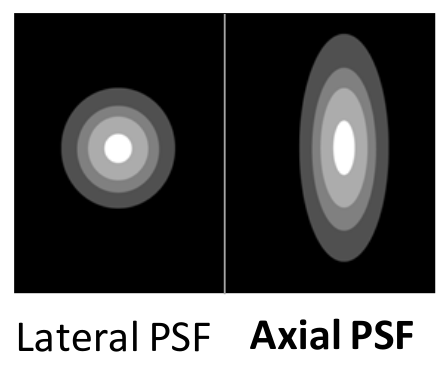
\includegraphics[width=0.3\linewidth]{./img/spim_01_psf.png}
			\captionsetup{width=.8\linewidth}
			\caption{Une image des fonctions d'étalement de point (PSF) axiales et latérales en imagerie SPIM.}
			\label{img:spim_01_point_spread_function}
		\end{figure}
		% }}}

		% IMG : Configurations SPIM, schéma {{{
		\begin{figure}[!h]
		    \centering
		    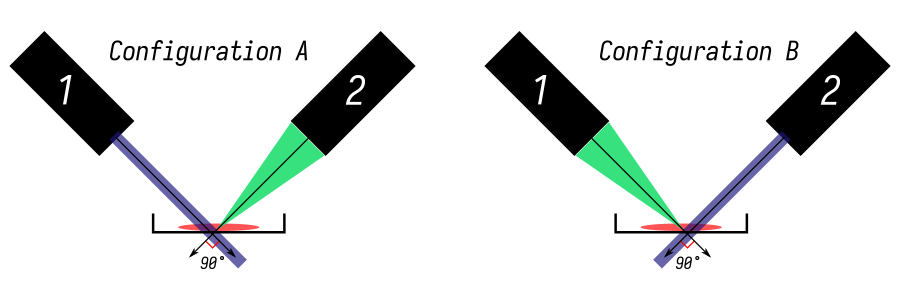
\includegraphics[width=.9\linewidth]{img/config_spim.png}
		    \captionsetup{width=.8\linewidth}
		    \caption{Configurations possibles des capteurs \textit{SPIM} (simplifié). En orange, l'échantillon reposant dans un récipient quelconque. En configuration A, la capteur 1 sert d'émetteur de lumière, et le capteur 2 sert d'appareil de capture. En configuration B, les rôles sont inversés.}
		    \label{img:spim_config}
		\end{figure}
		% }}}

		Dans cette méthode, il existe donc deux dispositifs \textit{SPIM} qui servent tour à tour de capteur, puis d'émetteur. Ces deux dispositifs sont placés à angle droit l'un de l'autre (voir figures \ref{img:lsm_02_device} et \ref{img:spim_config}), au dessus de la plateforme sur laquelle on dépose l'échantillon transparisé à analyser. Le fait d'avoir deux dispositifs \textit{SPIM} permet d'éliminer l'anisotropie de la fonction d'étalement de point dans les captures en combinant les acquisitions des capteurs depuis leurs points de vue différents, grâce à l'utilisation d'une opération de déconvolution\definition{Opération visant à restaurer le signal originel à une acquisition}.
		
		Le microscope \textit{di-SPIM} enregistre donc chacune des acquisitions d'un capteur dans une pile de coupes, qui sont discrétisées, quantifiées et enregistrées en tant qu'images traditionnelles au format \texttt{TIFF}, et qui nous est ensuite remise pour l'analyser et reconstruire un modèle tridimensionnel par la suite.
	}
	% }}}
	
	
    % Section jeux de données {{{
    \section{Présentation du jeu de données}\label{section:dataset}
    {
        Comme expliqué dans la section précédente, le microscope de l'université de Tulane possède deux capteurs disposés en angle droit l'un par rapport à l'autre. Ainsi, lors d'une acquisition d'un échantillon, le microscope capture des coupes à $\pm~\ang{45}$ par rapport à l'échantillon. Pour le système d'acquisition du microscope, cet échantillon est un signal continu tridimensionnel, comme représenté dans la figure \ref{img:spaces_real_initial}\texttt{(A)}. Ainsi, afin d'être enregistré, puis par la suite analysé il faut tout d'abord faire une discrétisation de ce signal, suivie d'une quantification de celui-ci. Ces deux étapes sont dépendantes des caractéristiques techniques du capteur (figure \ref{img:spaces_real_initial}\texttt{(B)}). Les images sont ensuite enregistrées sur disque, ce qui équivaut à leur appliquer une transformation (cisaillement) qui les place dans un repère orthonormé (voir figure \ref{img:spaces_real_initial} \texttt{(C)}). Dans cette configuration, l'échantillon est effectivement déformé par la transformation subie lors de l'enregistrement des images. Afin de le reconstruire, il nous sera nécessaire d'inverser cette transformation.

        Ces paires d'empilements d'images forment les différents jeux de données qui seront mis à notre disposition. Le microscope étant toujours en développement, ses caractéristiques techniques peuvent encore changer. La résolution des capteurs ainsi que le degré d'agrandissement fourni par le système optique pouvant évoluer dans le futur, il nous faudra pouvoir nous adapter à un tel changement.

        \begin{figure}[h]
            \centering
            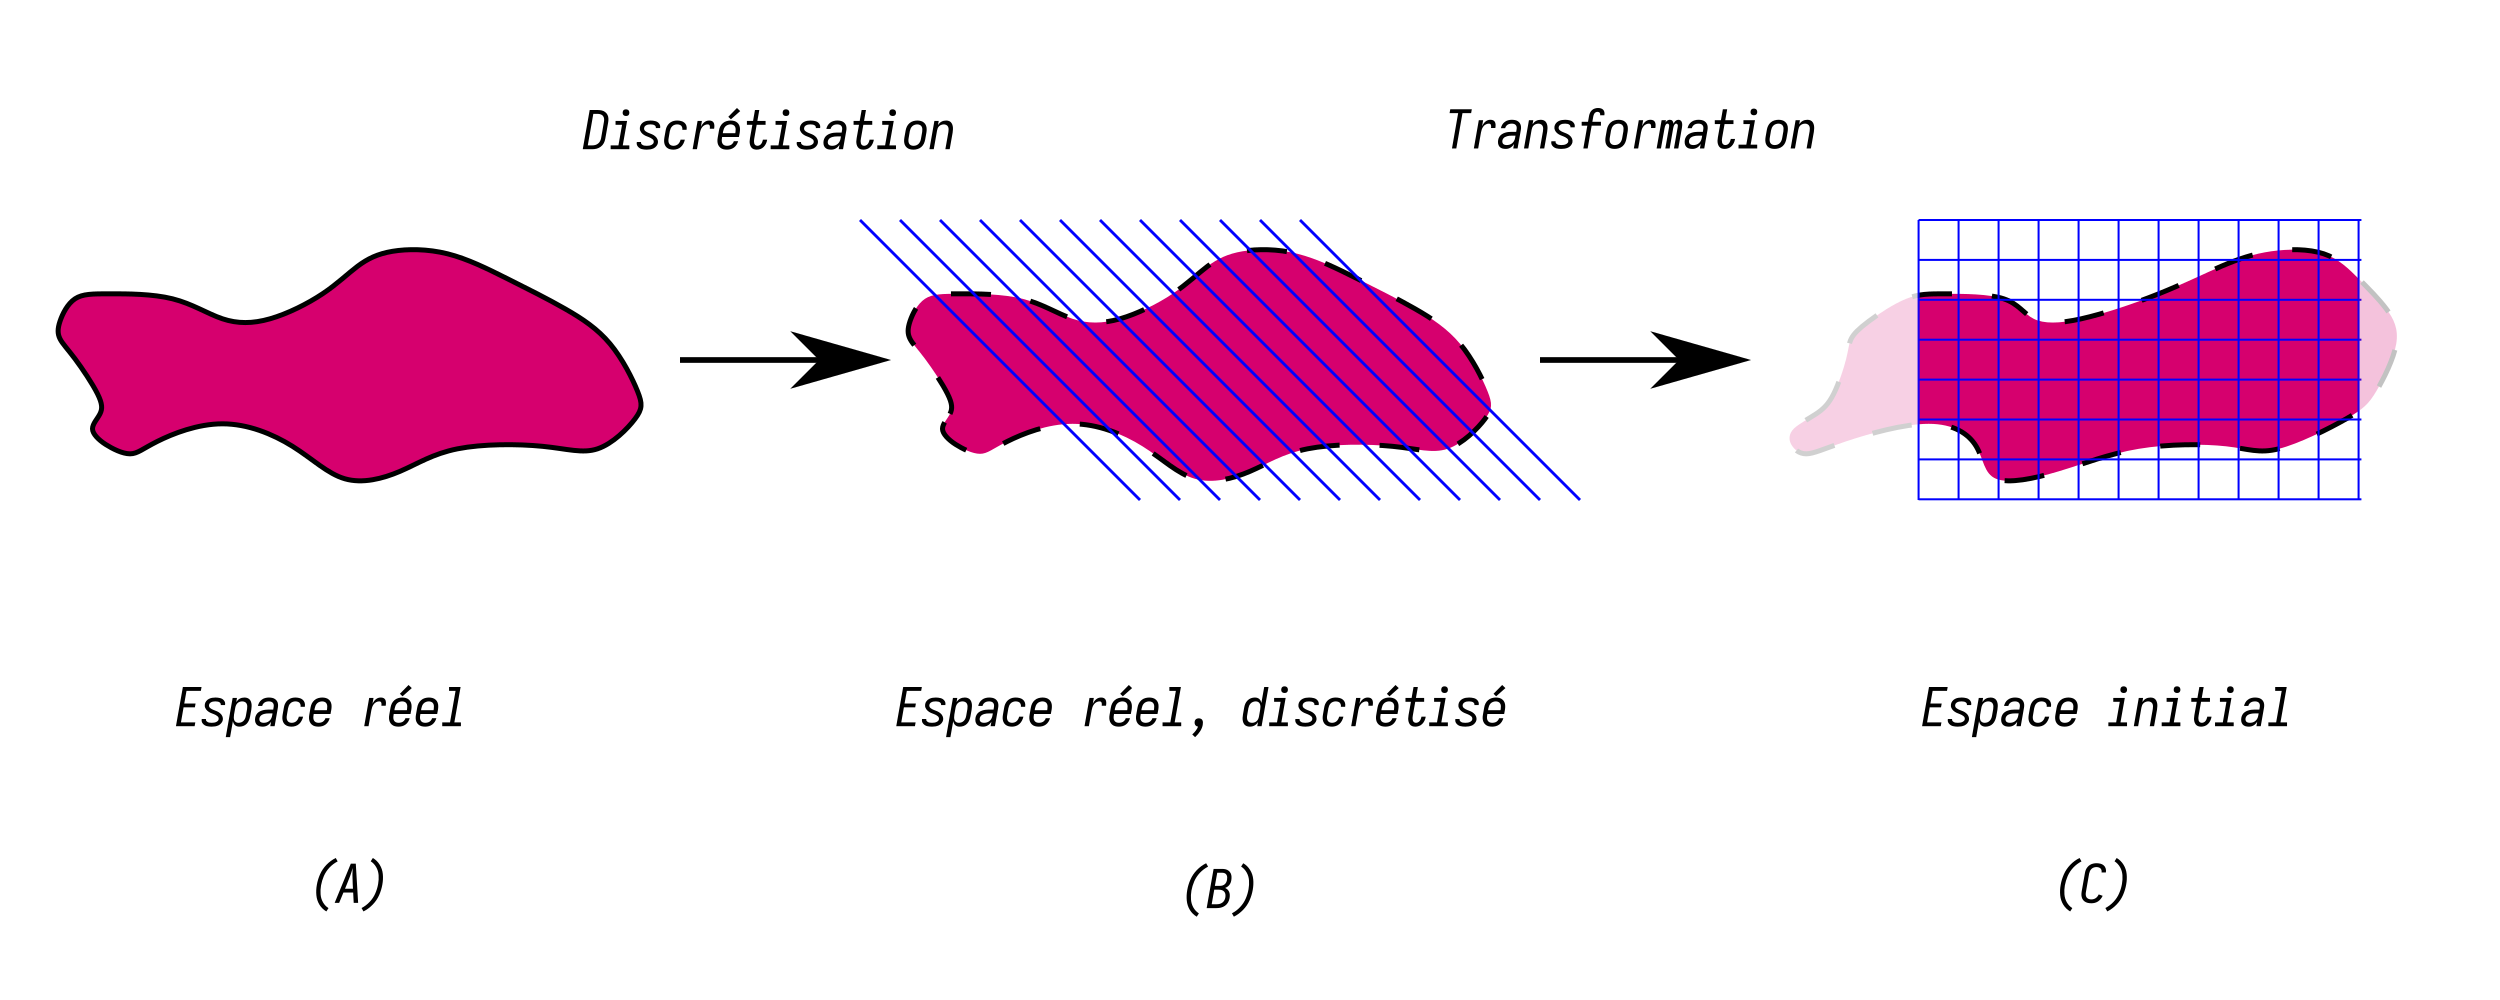
\includegraphics[width=\linewidth]{img/spaces_transfo_1_updated.png}
            \captionsetup{width=.8\linewidth}
            \caption{Différents espaces et transformations définis pour le programme. En magenta, l'échantillon à analyser. En bleu au centre, les différentes prises de vues effectuées par un capteur sur cet échantillon. En bleu à droite, la pile d'images résultante.}
            \label{img:spaces_real_initial}
        \end{figure}

        Afin de capturer un échantillon, le microscope effectue un ou plusieurs "balayages" du tissu (un exemple de plusieurs balayages est conceptualisé en figure \ref{img:multiple_image_captures}), afin de acquérir la totalité de celui ci. Chacune de ces captures sont constitués de deux piles d'images. En effet, comme vu en section~\ref{section:microscopy} la méthode de \textit{di-SPIM} utilise deux capteurs, orientés perpendiculairement l'un par rapport à l'autre. Le microscope est capable de prendre des acquisitions de l'échantillon contenant jusqu'à 20000 prises de vues. Ainsi, nous devons proposer des méthodes de traitement des données pour la visualisation et la reconstruction adaptées à ces jeux de données massifs.

        \begin{figure}[h]
            \centering
            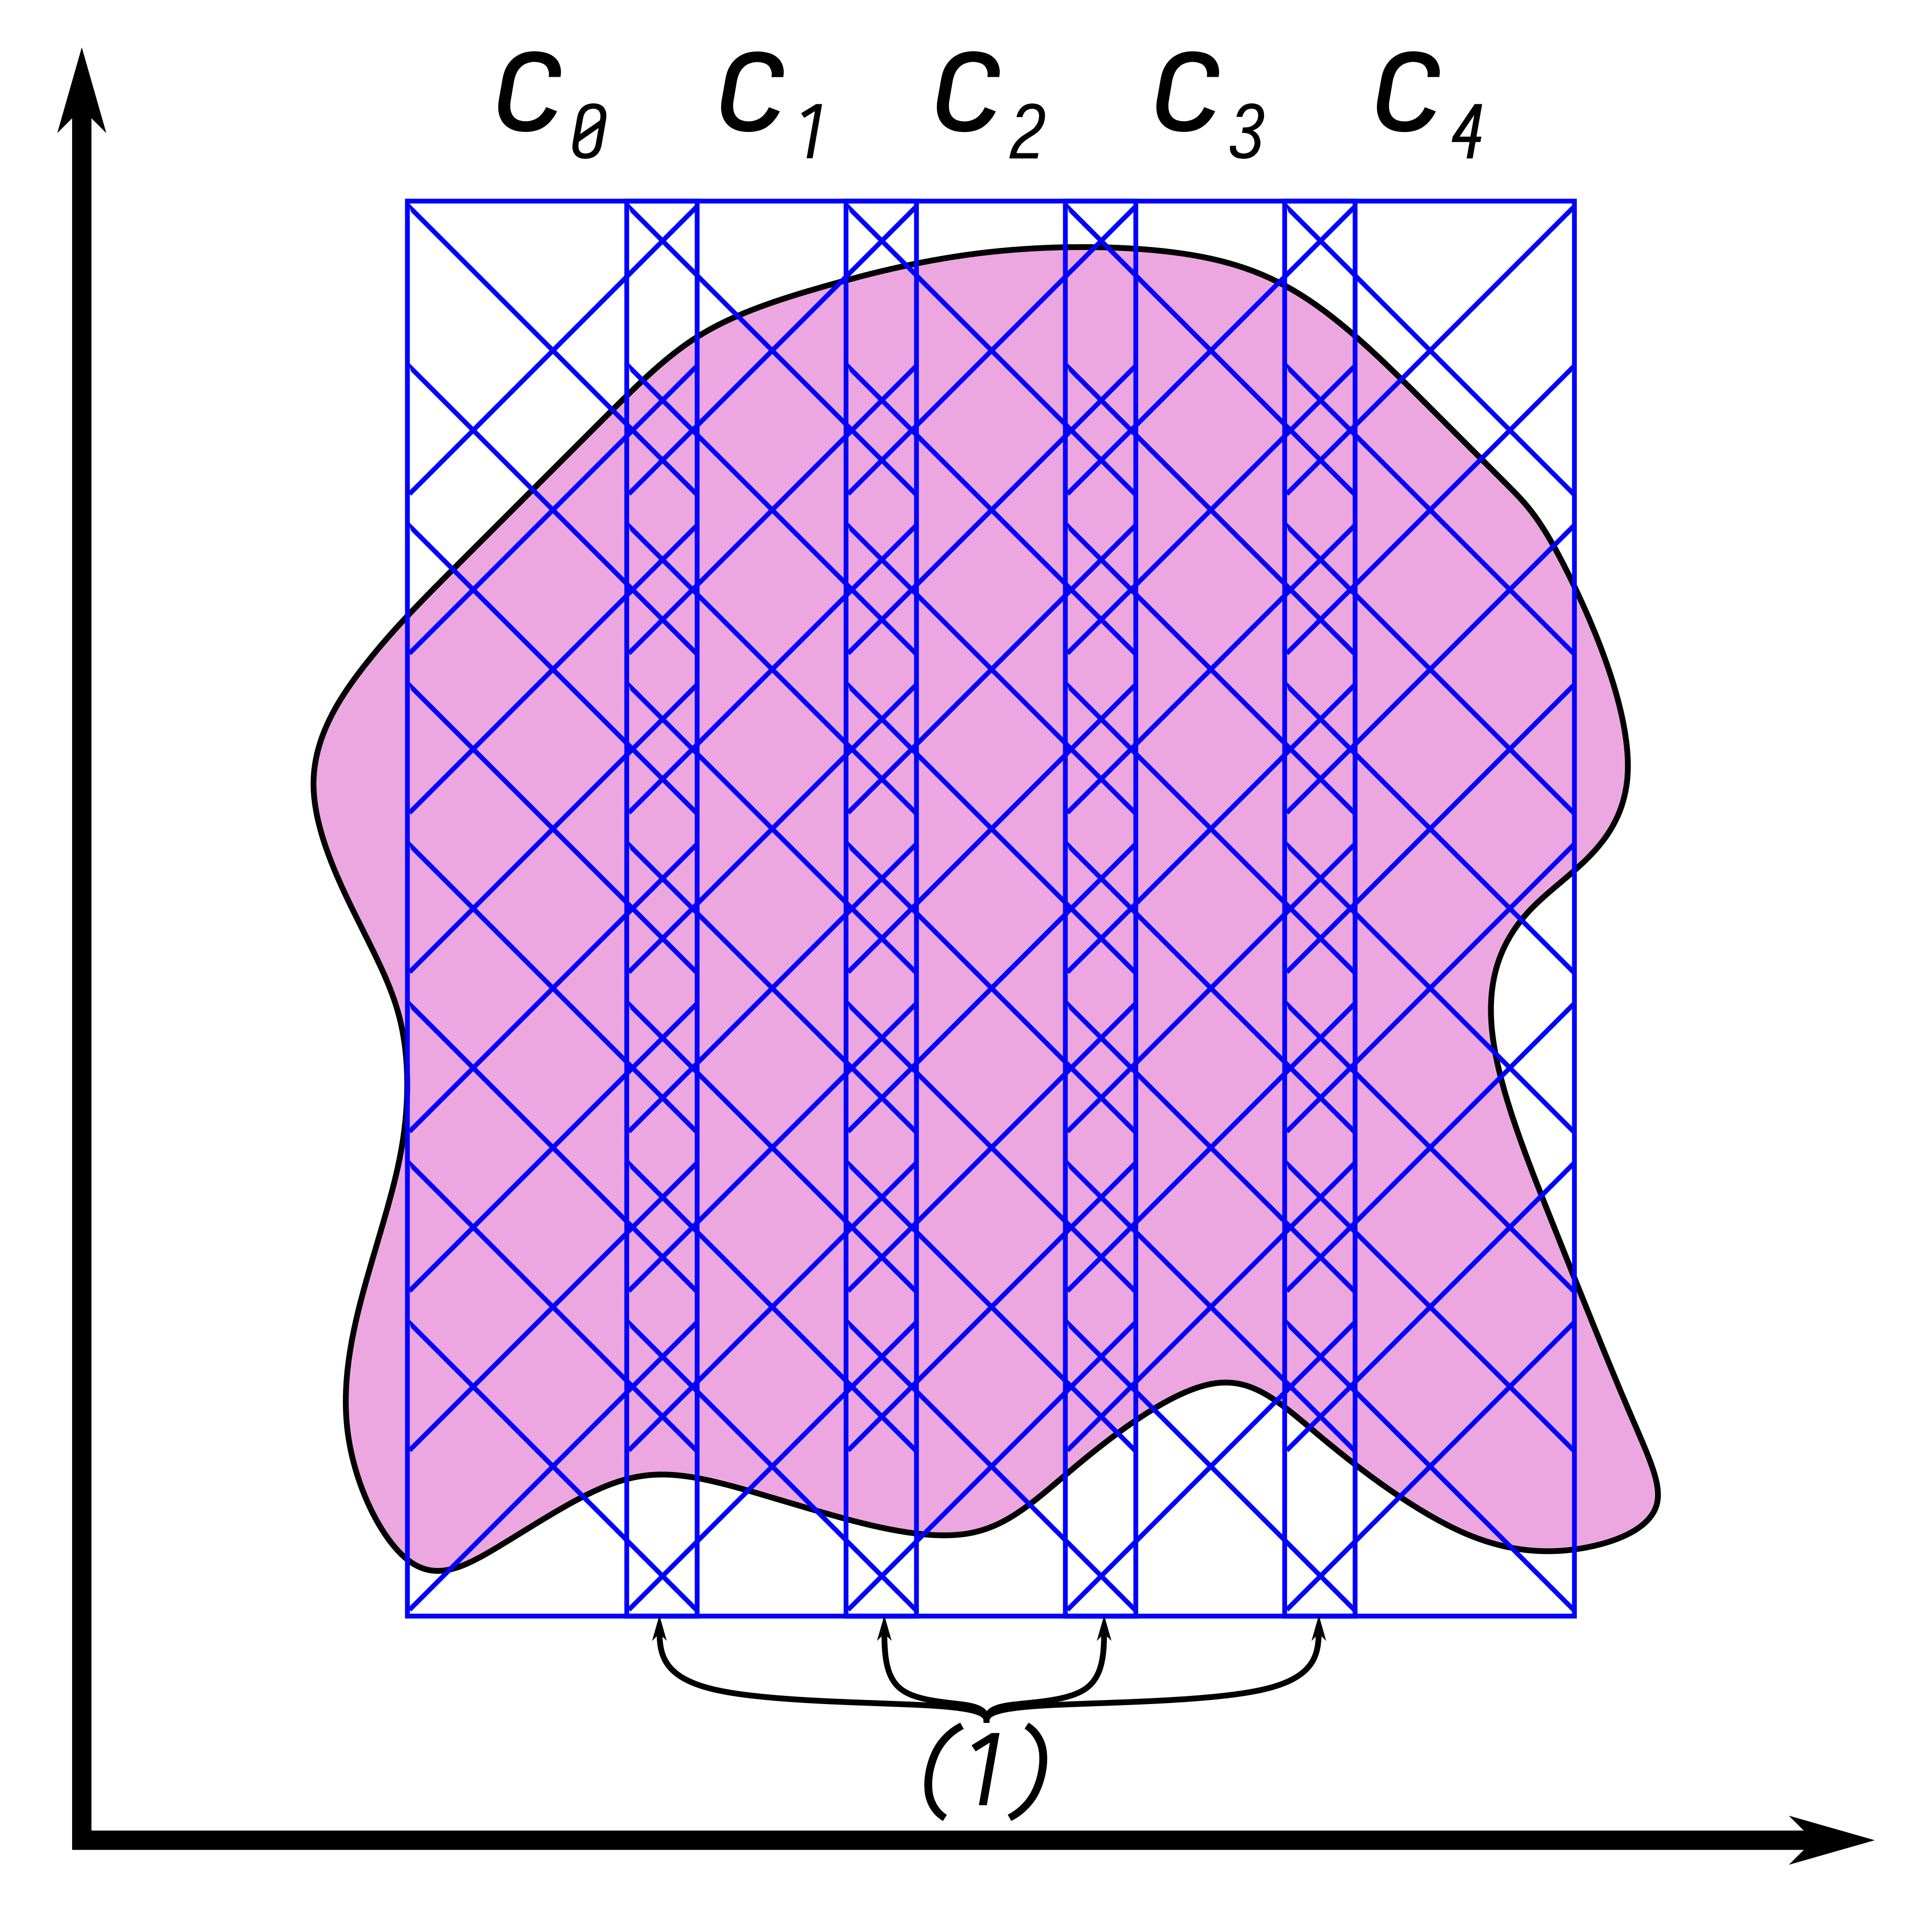
\includegraphics[width=.5\linewidth]{img/multiple_captures.png}
            \captionsetup{width=.7\linewidth}
            \caption{Un exemple d'acquisition d'un échantillon via de multiples captures. Chacune de ces captures (de $c_0$ à $c_4$) produira deux piles de $n$ images. Les captures présenteront des zones de chevauchement comme montré en (1).}
            \label{img:multiple_image_captures}
        \end{figure}

        Nous travaillons sur un jeu de données résultant d'une acquisition de tissu de prostate, composé d'une paire de piles d'images de 2000 images chacune. Les images sont de résolution $2048~\times~2048$, et sont en niveaux de gris sur 8 bits, résultant en une acquisition d'environ 16 gigaoctets. Ces piles d'images sont séparées en plusieurs fichiers \texttt{TIFF} contenant chacun une coupe uniquement. Un exemple d'un de ces fichiers peut être visualisé en figure \ref{img:data:both_prostate_samples}.

        \begin{figure}[ht]
            \centering
            \begin{tabular}{ccc}
                \begin{subfigure}[t]{.45\linewidth}
                    \centering
                    
\includegraphics[width=.8\linewidth]{img/tulane_data/prostate_tulane.png}
                    \captionsetup{width=.8\linewidth}
                    \caption{Tissus de prostate, tels que capturés depuis le microscope}
                    \label{img:data:prostate}
                \end{subfigure}& \hfill &
                \begin{subfigure}[t]{.45\linewidth}
                    \centering
                    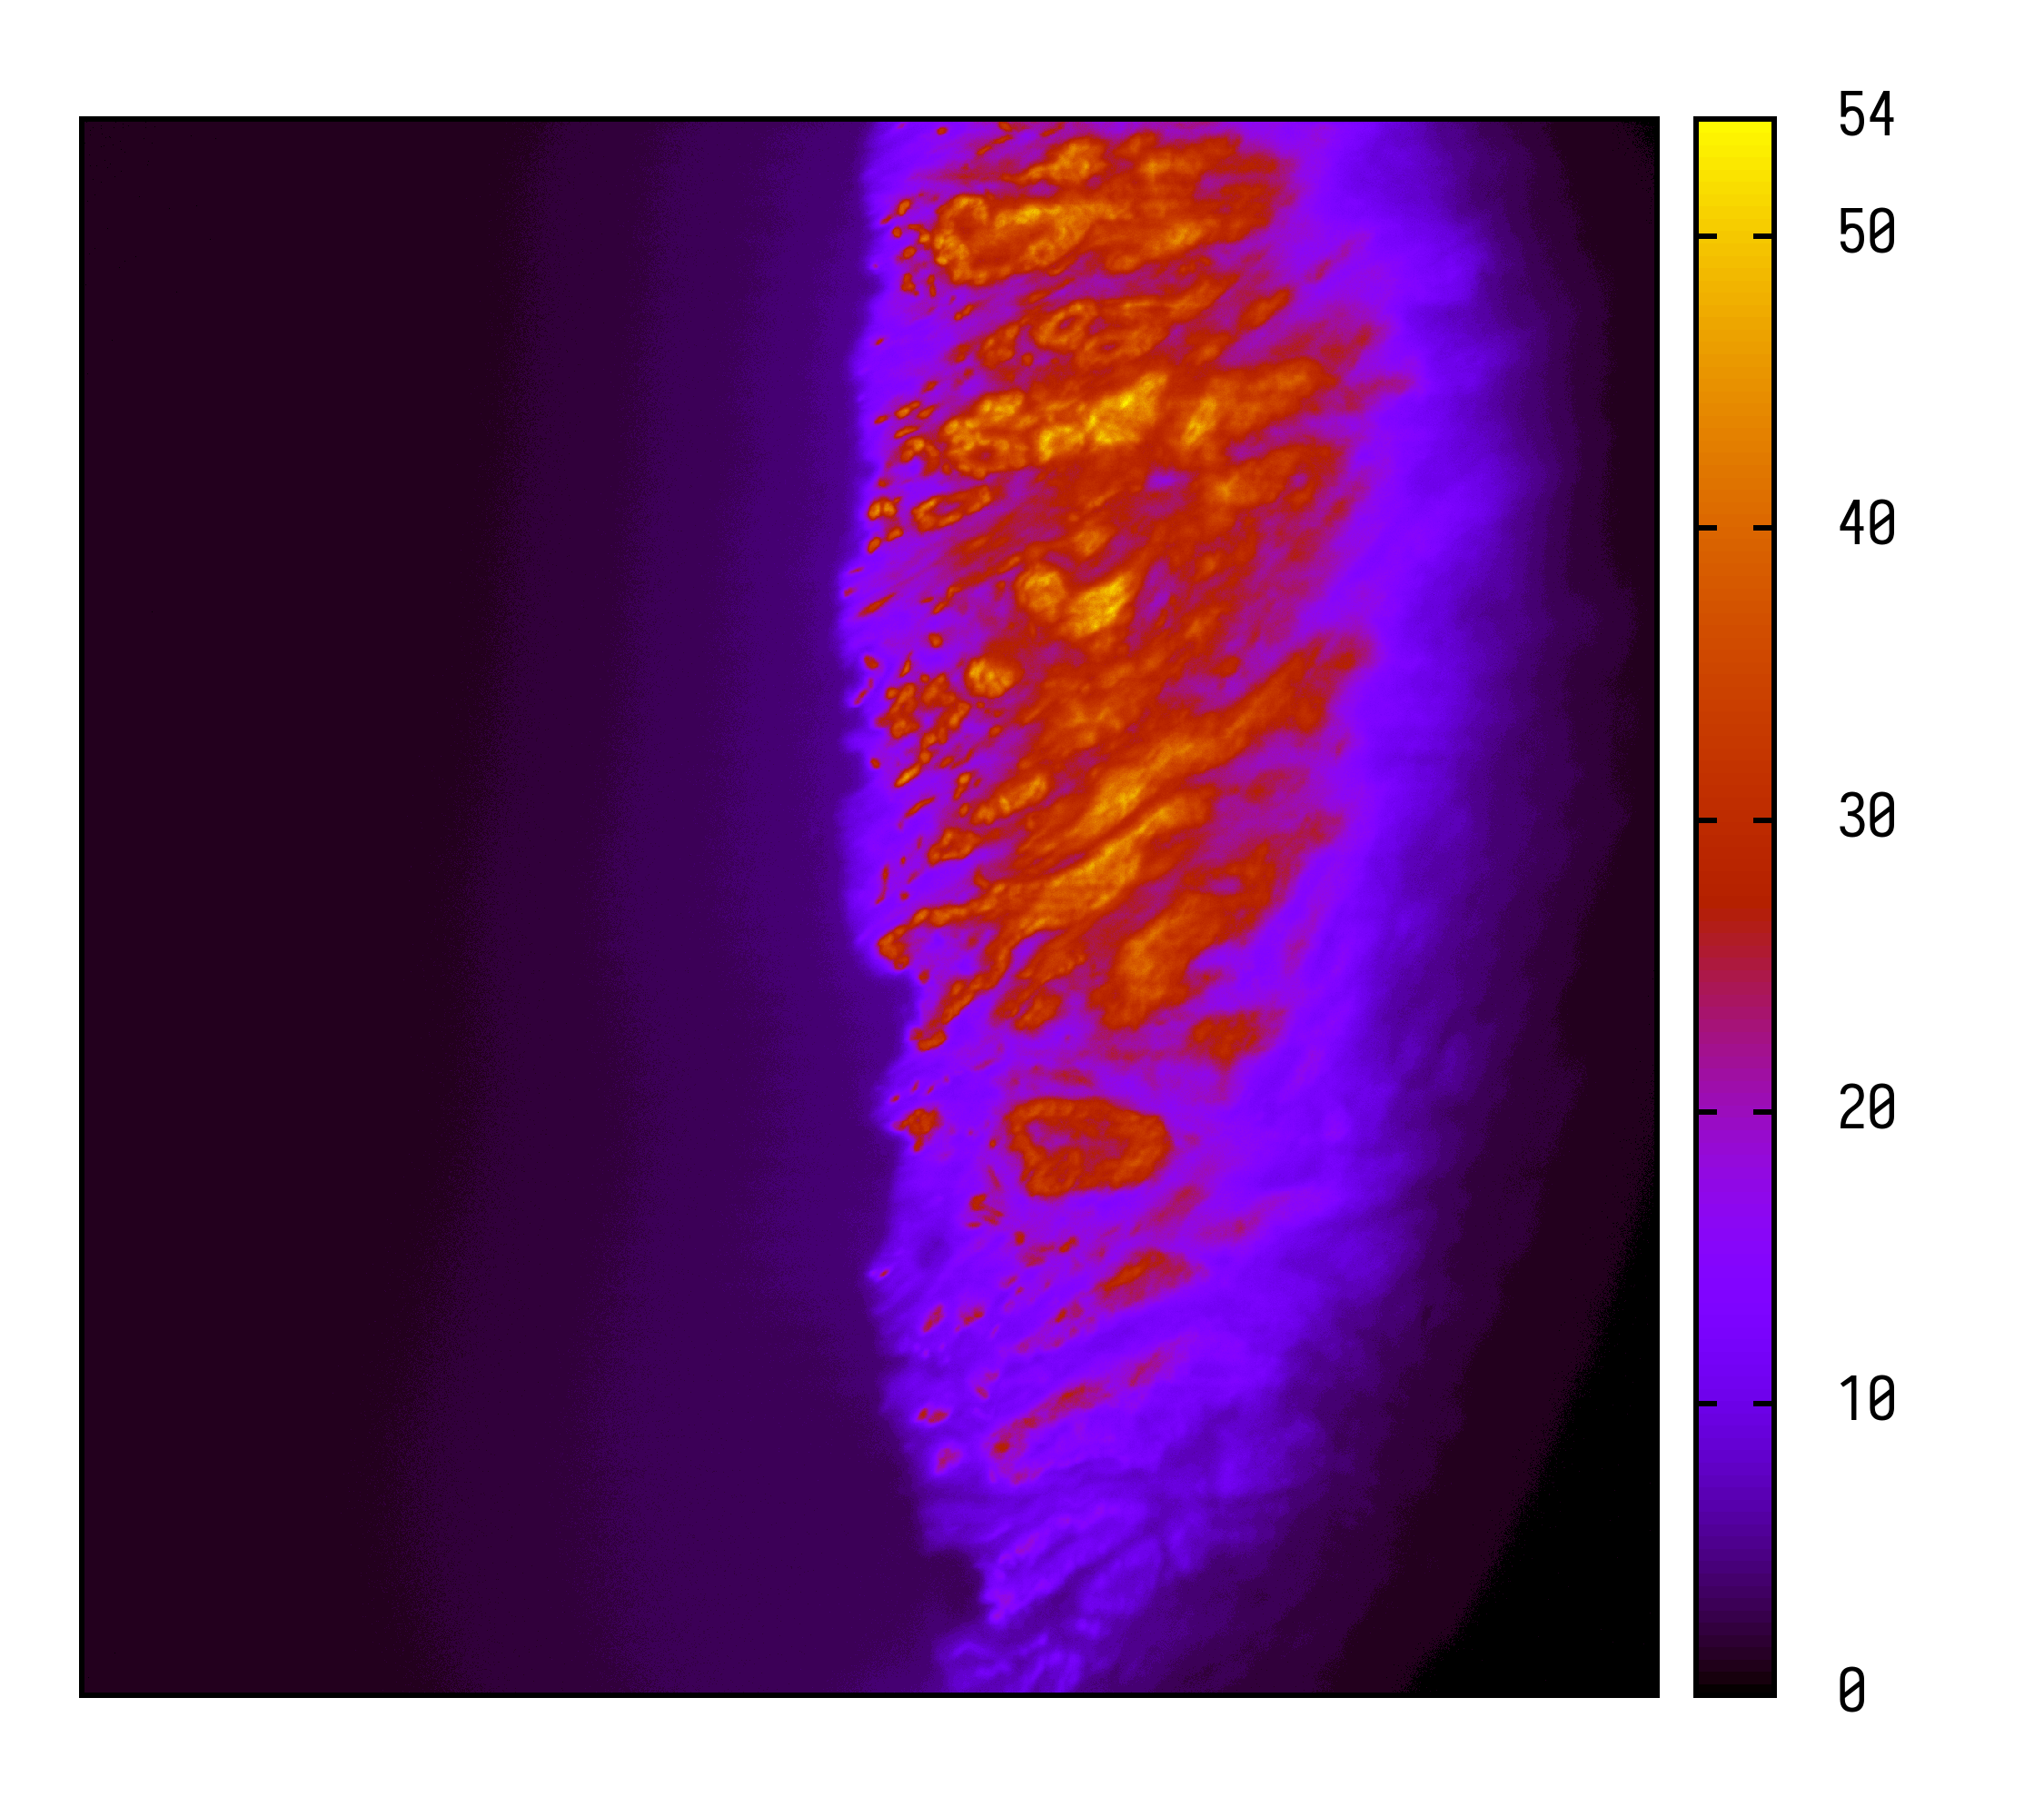
\includegraphics[width=.99\linewidth]{img/tulane_data/prostate_data_colourized.png}
                    \captionsetup{width=.8\linewidth}
                    \caption{Tissus de prostate, colorisé par \texttt{gnuplot} selon les valeurs de gris.}
                    \label{img:data:prostate_coloured}
                \end{subfigure}
            \end{tabular}
            \captionsetup{width=.8\linewidth}
            \caption{Acquisitions réalisées à l'université de Tulane, utilisées pour ce stage.}
            \label{img:data:both_prostate_samples}
        \end{figure}

        Nous pouvons voir qu'une grande partie de cette image (et plus généralement des autres images présentes dans ce jeu de données) est constituée de valeurs faibles, sur les côtés de l'échantillon. Les chercheurs à Tulane nous ont informés que lors de l'enregistrement des images, nous devions considérer les valeurs inférieures à 5 comme du bruit de fond, ne représentant pas aucune information. Ainsi, une grande partie de cette image ne contient aucune donnée significative pour notre cas d'utilisation.

        En analysant les coupes présentes dans ce jeu de données, nous pouvons voir dans la figure \ref{img:prostate:stats} que près de $70\%$ des données sont à considérer comme du bruit. La figure \ref{img:prostate:stats:repartition} représente la probabilité qu'un pixel aléatoire dans le jeu de données soit supérieur à $n$. Si l'on prend $n = 5$, nous pouvons voir que uniquement $31\%$ des données présentes représentent une information utile à la reconstruction. De plus, nous pouvons remarquer que le contraste de ces images n'est pas extrêmement élevé, ce qui pourra poser problème lorsque l'on devra faire des analyses de forme de la structure d'un échantillon.
        
        En effectuant une reconstruction partielle des images chargées en mémoire, nous pourrons donc économiser non seulement beaucoup de place mémoire, mais également raccourcir le temps nécessaire pour une reconstruction complète de l'échantillon.

        Le choix de mettre les acquisitions en format \texttt{TIFF} est judicieux, car ce format permet une grande flexibilité pour le format d'images enregistrées : il est possible d'étendre le format originel par le biais d'extensions, permettant d'enregistrer plus d'informations sous des formats quelconques, et c'est la responsabilité de l'application de lecture des images à implémenter le support de ces extensions ou non.
        
        \begin{figure}[H]
            \centering
            \begin{subfigure}{.8\linewidth}
                \centering
                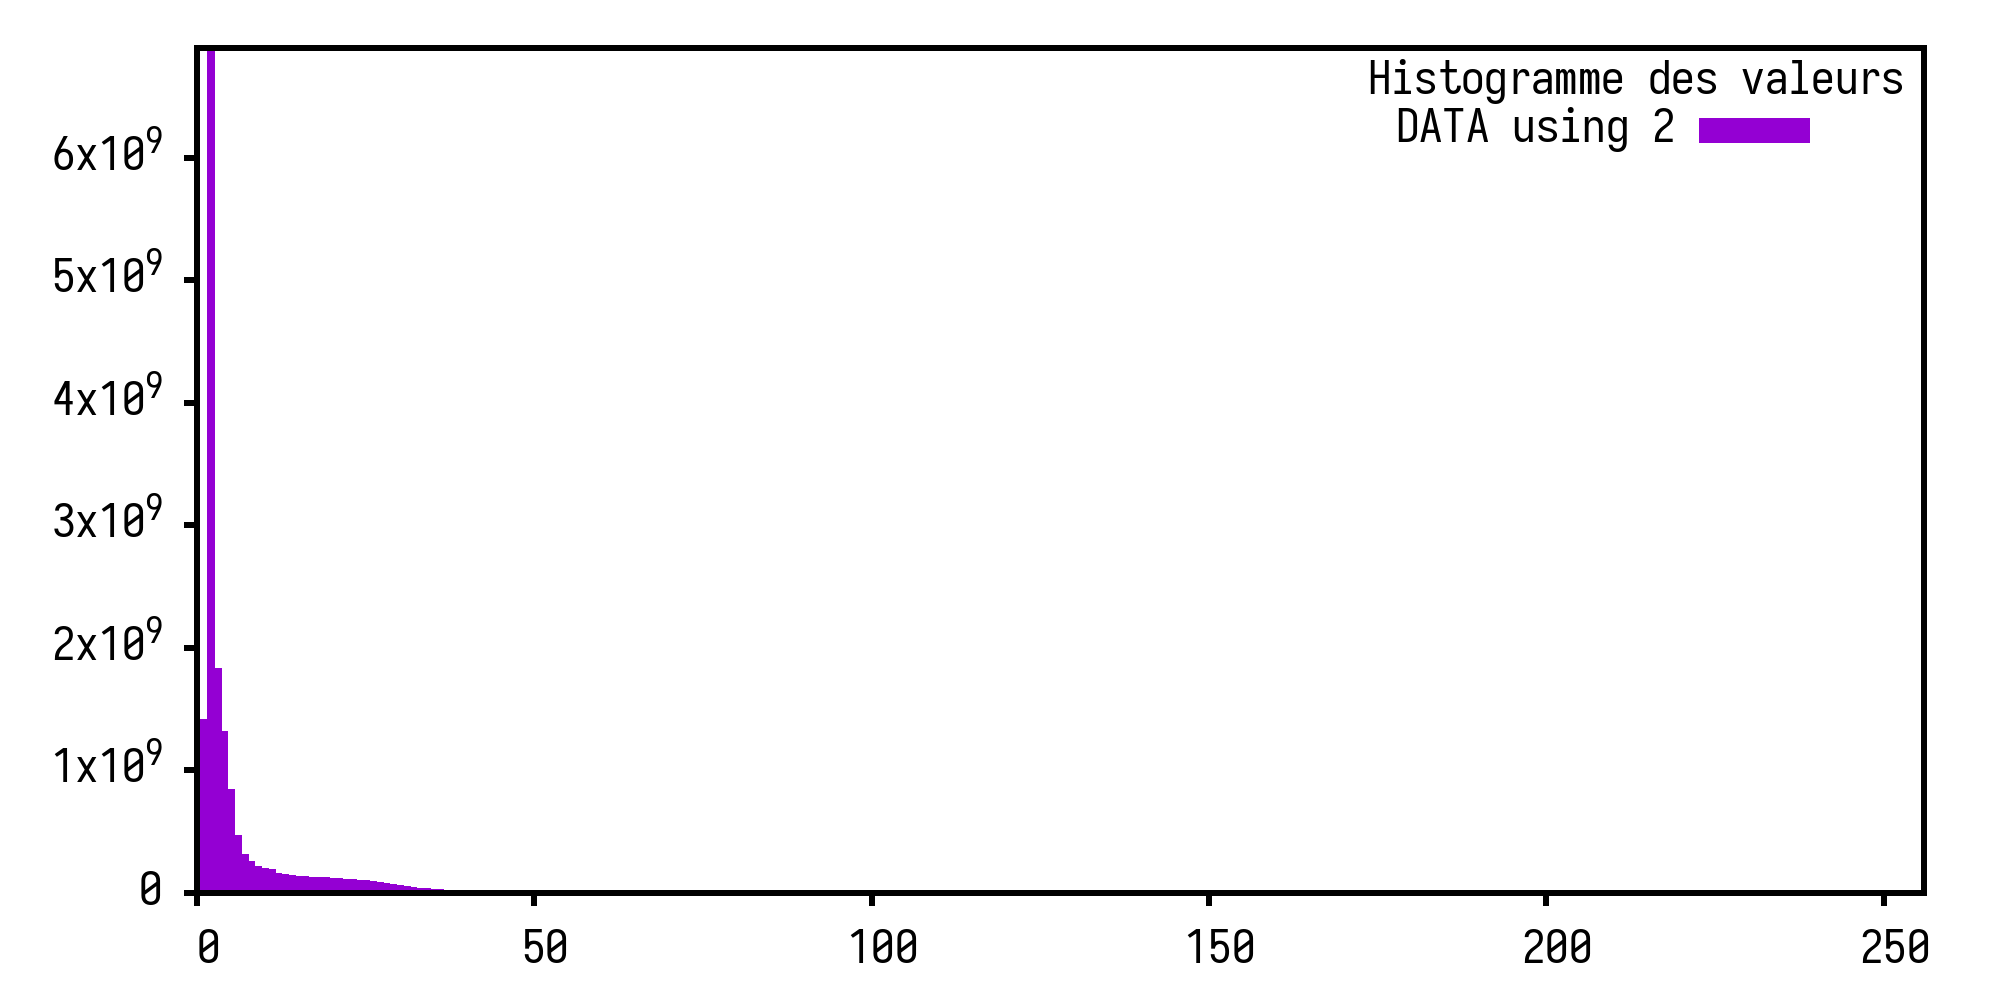
\includegraphics[width=\linewidth]{img/stats/histo.png}
                \caption{Histogramme des valeurs de niveaux de gris présentes dans le jeu de données}
                \label{img:prostate:stats:histogram}
            \end{subfigure}
            \begin{subfigure}{.8\linewidth}
                \centering
                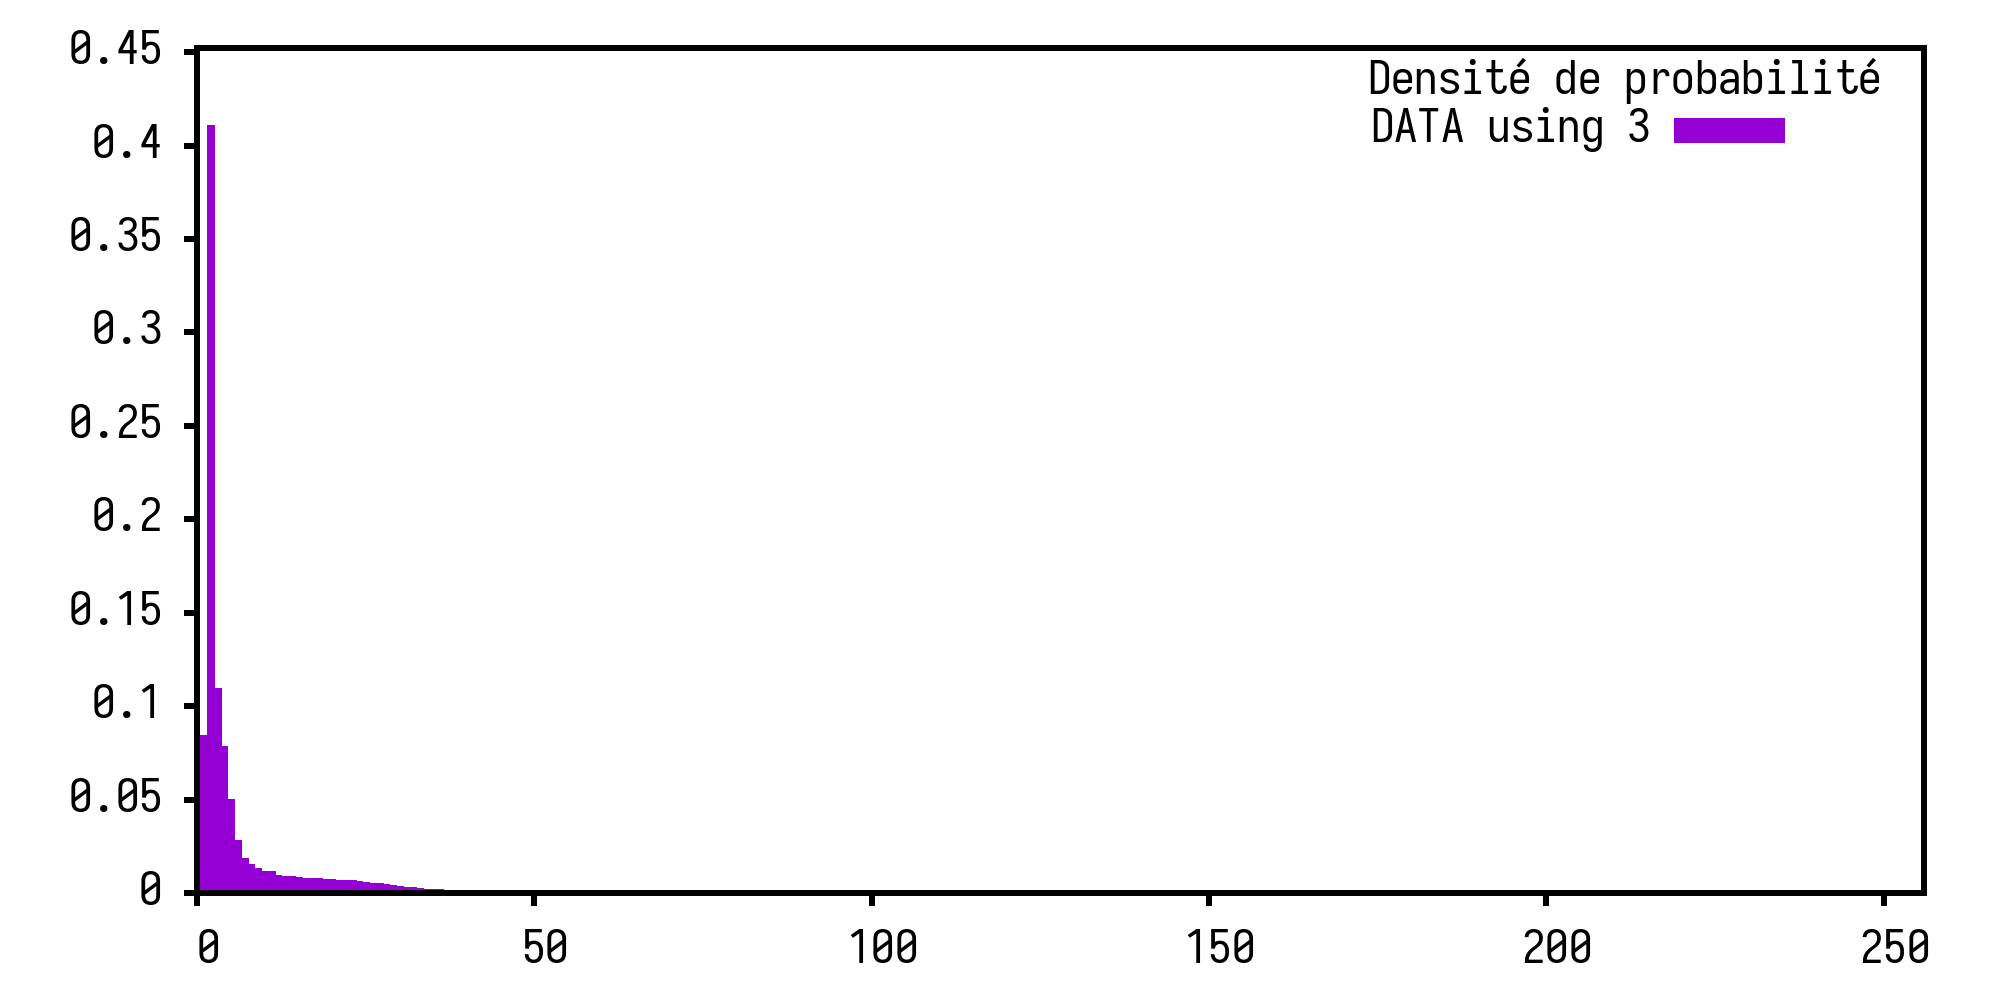
\includegraphics[width=\linewidth]{img/stats/distrib.png}
                \caption{Densité de probabilités des valeurs de niveaux de gris du jeu de données}
                \label{img:prostate:stats:ddp}
            \end{subfigure}
            \begin{subfigure}{.8\linewidth}
                \centering
                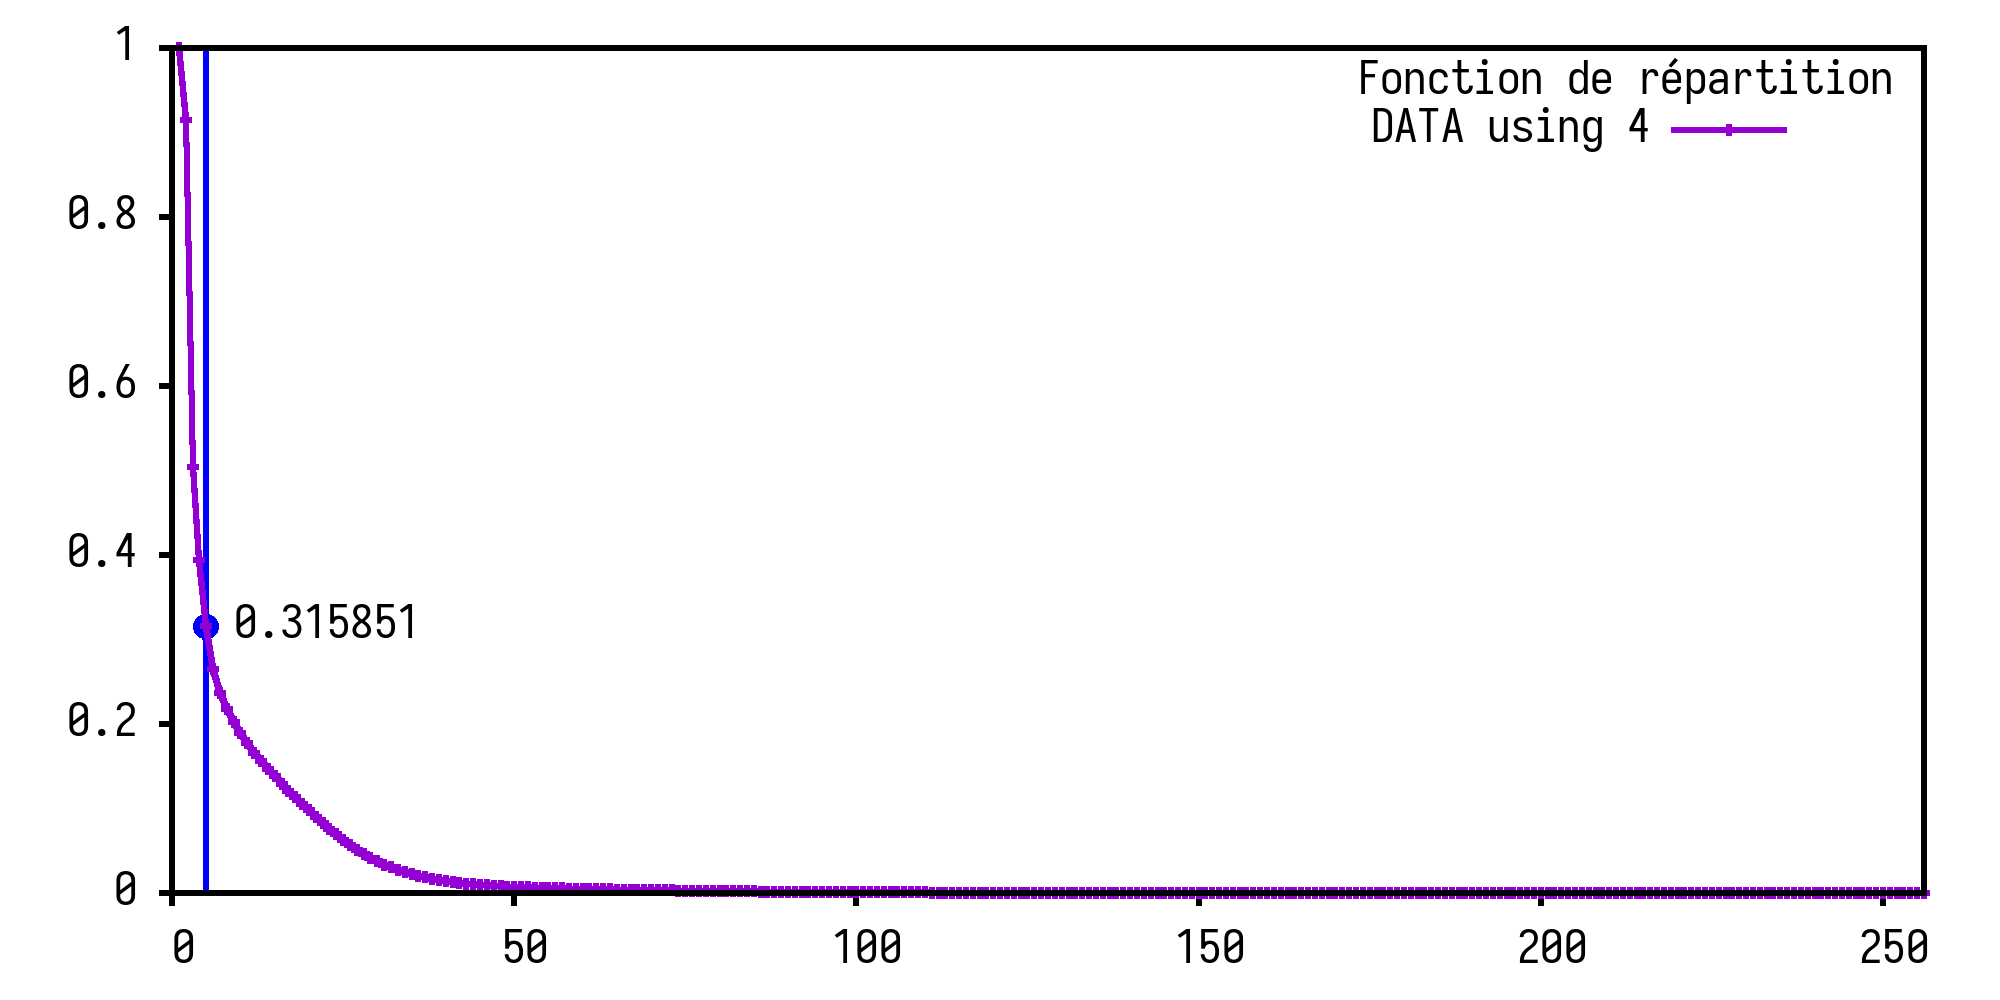
\includegraphics[width=\linewidth]{img/stats/proba.png}
                \caption{Fonction de répartition (inversée) des valeurs de niveaux de gris dans le jeux de données. La droite bleue à $x~=~5$ est permet de visualiser quelle proportion des données sont utiles dans l'acquisition de l'échantillon.}
                \label{img:prostate:stats:repartition}
            \end{subfigure}
            \captionsetup{width=.8\linewidth}
            \caption{Quelques informations sur le jeu de données fourni par Tulane}
            \label{img:prostate:stats}
        \end{figure}
        
        Une capture étant composée d'un empilement de coupes de l'échantillon de même résolution, celle-ci est donc représentée comme une image 3D, communément représentée comme une grille volumique orthonormée dont tous les éléments sont appelés \textit{voxels}, l'analogue du pixel en trois dimensions. Cette structure de données possède quelques avantages et inconvénients qui seront explorés plus en profondeur dans la section \ref{section:voxelgrid}. Cette représentation de l'acquisition de l'échantillon est une forme primaire de reconstruction 3D. Mais dans notre cas, celle-ci ne prend pas en compte les spécificités apportées par la méthode d'acquisition \textit{di-SPIM}, et ne permet pas non plus une étude de la forme des glandes dans l'échantillon car celui-ci est déformé dans son état actuel.
    }
    % }}}
    
    % Section Tulane {{{
	\section{Pré-traitement des données}\label{section:previous_tulane_work}
	{
	    %Le microscope développé par les chercheurs de l'université de Tulane permet d'effectuer une acquisition d'échantillon en utilisant la méthode \textit{di-SPIM} (détaillé en section \ref{section:microscopy}), effectuant une acquisition par coupes de l'échantillon, de manière non destructive. Chacune de ces coupes est transformée en image puis empilée avec les autres coupes de ce capteur, résultant en une image 3D. %Dans les travaux présentés ci-après dans le rapport, nous ne nous intéresserons pas au bruit présent sur le signal capturé, car la création d'un modèle de bruit ne rentre pas dans le cadre du stage.
	    
	    Dès l'arrivée des première acquisitions, les chercheurs de l'université de Tulane ont mis en place une méthode, non optimisé, de reconstruction volumique de l'échantillon. % ne prenant pas en compte les spécificités amenées par la technique de microscopie \textit{di-SPIM}. 
	    Ce processus est composé de plusieurs étapes:
	    \begin{enumerate}
	    \item "redresser" les deux piles d'images entre elles en appliquant une transformation (cisaillement, rotation, troncature) sur chacune des coupes de l'image. Comme le montre les étapes $(C)$, $(D)$ et $(E)$ de la figure \ref{img:tulane_process:reconstruction}, la décomposition de cette transformation génère une consommation mémoire importante par le stockage de résultats intermédiaires non indispensables.
	    \item re-échantillonner les deux piles d'images pour avoir une résolution uniforme. %Une copie de chaque image est faite à cette étape.
	    \item fusionner les deux piles par une opération de déconvolution à double vue~\cite{cite_deconv_richardson_lucy, cite_deconv_spim_huisken}. Cette opération permet d'améliorer la qualité et la netteté de l'image capturée, en intégrant les données des deux piles d'images. 
	    \end{enumerate}
	    	    %, indépendantes les unes des autres, est coûteux en temps de calcul et gourmand en espace disque:
	    %Ce processus est long car chacune des opérations de transformation de l'image 3D est accompagnée d'un re-échantillonnage de cette image afin de pouvoir avoir des données uniformément échantillonnées. Ces enchaînements d'interpolations suivies d'opérations complexes entraînent une explosion des quantités de données nécessaires pour stocker une acquisition complète. 
	    Chacune de ces opérations menant à une reconstruction de l'échantillon prennent plusieurs heures, et génèrent jusqu'à plusieurs téraoctets de données afin d'obtenir un résultat correct. Ces choix algorithmiques sont justifiés en grande partie par l'emploi de logiciels comme \texttt{ImageJ} ou \texttt{Amira} et de langage scriptés non optimisés tels que \texttt{Matlab} par des utilisateurs non experts. La contribution majeur de ce travail est de fournir une solution méthodologique et logicielle adaptée permettant d'effectuer ces traitements de façon économe et efficace en mémoire. De plus, notre système permet la visualisation interactive de la structure tridimensionnelle des glandes de la prostate.  % et faite à la volée, nous pouvons effectuer ces traitements plus rapidement, tout en utilisant moins de mémoire que la solution actuelle. De plus, les algorithmes étant adaptés au cas particulier de la microscopie \textit{di-SPIM}, nous pouvons conserver la morphologie complexe de l'échantillon de tissu afin de l'analyser par la suite.
	}
	    
	    \begin{figure}[h]
	        \centering
	        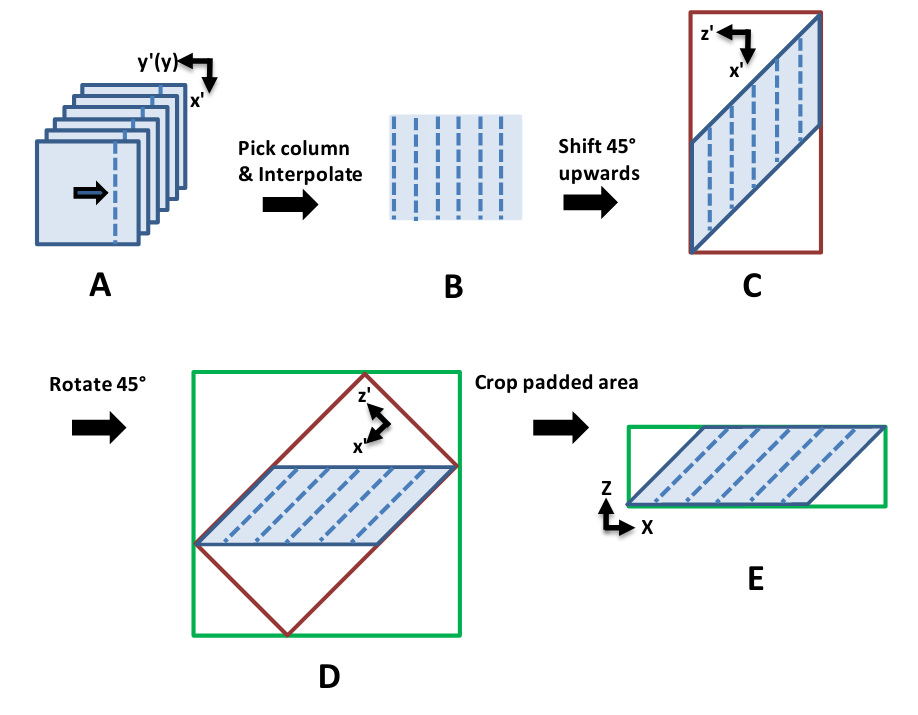
\includegraphics[width=.65\linewidth]{img/tulane_process.png}
	        \captionsetup{width=.8\linewidth}
	        \caption{Le processus actuel de reconstruction de l'université de Tulane, sans la partie de déconvolution.}
	        \label{img:tulane_process:reconstruction}
	    \end{figure}
	    
	    
    %}}}
    
}
% VIM modeline : do not touch !
% vim: set spell spelllang=fr :

	% Contents of chapter 3
\chapter{Gestion et visualisation d'images}\label{chapter:03:memory_and_vis}
{
	% Plan {{{
	\commentaire{
		\begin{enumerate}
			%% gestion images en mémoire {{{
			\item intro : chargements d'images, recherche de voisins et génération de grille. prés du problème plus en détail
			\item travaux sur le chargement d'images\begin{enumerate}
				\item formats de sortie du microscope
				\item problème de tailles $\rightarrow$ downsampling
				\item recherche de librairies
				\item comparaison (très rapide) libtiff / tinytiff
				\item gestion de mémoire~\begin{itemize}
					\item downsampling à la volée des images, sur requête utilisateur
					\item parler de structure en mémoire une fois chargé
					\item on peut avoir autant d'images que on veut en mémoire
				\end{itemize}
				\item possibles travaux : buffer circulaire pour pas tout charger d'un coup et/ou chargement en multi-threading (a garder ici ou dans travaux à venir ?)
			\end{enumerate}
			% }}}
			\item visualisation plans de coupe
			%% KPF / Texture3D {{{
			\item Très rapide : intro à pourquoi on a fait ca :\begin{itemize}
				\item C'est un travail déjà presque entièrement fait, à tester et MàJ pour publication
				\item Ca peut nous servir d'une certaine façon pour visualiser le modèle en fin de stage
			\end{itemize}
			\item Présentation de la méthode (rapide, pas le focus du rapport)~\begin{itemize}
				\item Chargement de la texture
				\item Génération de maillage tétrahédrique à partir de maillage surfacique englobant (version binaire de la grille $\rightarrow$ maillage tétra, binariser grille $\rightarrow$ dilatation, et maillage autour de ca)
				\item (Rapide) Raymarching/Bresenham pour trouver voxel, et estimer normale et couleur
				\item Note : mentionner le fait que du coup, la complexité revient à la taille du framebuffer, non de la grille
				\item Effet de bord : on peut donc charger des grilles rentrant sur GPU, les déformer afin d'avoir une grille techniquement + grande que espace mémoire GPU
			%	\item Mentionner que ca va sortir à Vis 2020 si tout va bien
			\end{itemize}
			\item Présentation des travaux effectués (plus de détails, avec difficultés mentionnées)~\begin{itemize}
				\item Mise(s) à jour du code~\begin{itemize}
					\item 'Dépoussiérage' logiciel
					\item MaJ des shaders en GLSL : passé à qqchose de plus récent pour moins de problèmes incompatibilités
					\item Changement dans la gestion de la texture (vec4f $\rightarrow$ uchar + texture)
					\item Bug fixing pour grosses grilles
				\end{itemize}
				\item Tests de la méthode en vue de publication scientifique~\begin{itemize}
					\item Tests de performances
					\item Tests effectués sur grosses grilles
					\item Tests effectués sur petites grilles avec déformation
					\item Tests effectués à plusieurs résolutions
				\end{itemize}
				\item Difficultés encontrées sur le projet~\begin{itemize}
					\item Problème rencontré : incompatibilités Boost $\Leftrightarrow$ CGAL, et anciennes versions des libs $\Rightarrow$ problème de compilation
				\end{itemize}
			\end{itemize}
			\item Présentation des possibilités d'utilisation de la méthode dans notre cas~\begin{itemize}
				\item Une fois reconstruction effectuée, si taille grille générée $<$ taille mémoire GPU, alors possiblité de voir interactivement le modèle
				\item Générer une visu multi échelle avec fichiers comme H5F/HF5 afin de pull des infos qu'on a besoin : petit modèle sur GPU, et charger hiérarchiquement en zoomant progressivement
			\end{itemize}
			% }}}
		\end{enumerate}
	}
	% }}}

	% Prelude : présentation chapitre {{{
	Comme vu dans le chapitre précédent, nos collaborateurs à l'université de Tulane possèdent une méthode non destructive pour acquérir un échantillon de tissu humain à très haute résolution. Cette haute résolution, bien que préférable afin de pouvoir observer les fins détails du tissu, posent un problème : les données issue d'une acquisition sont très souvent massives et donc difficiles à gérer. Avec l'expertise que possède l'université de Montpellier dans le traitement d'images, nous pouvons leur prêter main-forte afin de réduire l'empreinte mémoire de ces images tout en gardant toute l'information présente dans chacune d'entre elles. Ainsi, un des objectifs de ce stage étant la gestion de données massives, la première partie de ce chapitre sera accordé aux travaux réalisés sur la gestion de mémoire lors du traitement des informations. Par la suite, nous allons parler de deux techniques permettant la visualisation en temps réel de ces données.
	% }}}

	Comme vu dans le chapitre précédent, nos collaborateurs à l'université de Tulane possèdent une méthode non destructive pour acquérir un échantillon de tissu humain à très haute résolution. Cette haute résolution, bien que préférable afin de pouvoir observer les fins détails du tissu, posent un problème : les données issue d'une acquisition sont très souvent massives et donc difficiles à gérer. Avec l'expertise que possède l'université de Montpellier dans le traitement d'images, nous pouvons leur prêter main-forte afin de réduire l'empreinte mémoire de ces images tout en gardant toute l'information présente dans chacune d'entre elles. Ainsi, un des objectifs de ce stage étant la gestion de données massives, la première partie de ce chapitre sera accordé aux travaux réalisés sur la gestion de mémoire lors du traitement des informations. Par la suite, nous allons parler de deux techniques permettant la visualisation en temps réel de ces données.

	\section{Gestion de mémoire}
	{
		\wip{Gestion de la mémoire dans ce cas là : permet de ne charger que les données nécessaires au traitement, afin de réduire temps de traitement \textsc{\textbf{et empreinte mémoire}}~}\\

		\commentaire{ne pas oublier de parler de comment les données sont structurées en mémoire une fois chargées}\\

		Afin de proposer une méthode de traitement des données générées par le microscope, il faut d'abord pouvoir gérer lesdites données. Cette partie étant intimement liée aux format de sortie des données provenant du microscope, il est important de rappeler les caractéristiques de celui-ci.\par

		L'équipe de Tulane nous a fait parvenir\todo{a redire de facon plus soutenue} quelques ensembles de jeux de données. Ceux-ci représentent quelques exemples d'échantillons acquis avec leur microscope. Ces exemples sont des images en niveaux de gris \wip{A finir, intro technique aux images et mentionner limite maximale au nb d'images en 1 stack dans les jeux de données}\par

		Avec des images de si haute résolution et en si grand nombre, il est nécessaire de pouvoir efficacement utiliser la mémoire disponible, afin de charger le plus de données possible. Il faut également un processus de chargement de ces images rapide, afin de ne pas attendre indéfiniment la lecture des données, mais aussi assez flexible pour permettre de gérer les différents types d'images que le microscope peut sortir\todo{maladroit, réécrire}. Les problèmes de taillent peuvent être résolus avec du sous échantillonnage, mais la problématique de la flexibilité et de la rapidité doivent être résolus\todo{conjugaison : vérifier} avec l'utilisation de librairies externes. Ainsi, nous comparerons plusieurs librairies : \texttt{libtiff} et \texttt{TinyTIFF}.\par

		\wip{Retrouver benchmark tinytiff/libtiff et mettre ici}\par

		Attaquons nous maintenant au problème de la gestion de la mémoire utilisée par ces images, lors du chargement, et une fois chargées.

		\subsection{Utilisation et disposition mémoire}\todo{changer titre}
		{
			Afin de permettre de la visualisation en temps réel, nous devons permettre à l'utilisateur de charger le plus d'images possibles en mémoire. La visualisation à l'oeil nu ne nécessitant pas d'avoir le maximum de résolution possible\todo{re-ecrire, maladroit}, nous proposons un pré-traitement des images, en les sous-échantillonnant, afin d'en faire rentrer le plus grand nombre en mémoire. Ainsi, une visualisation en temps réel est possible pour l'intégrité des images chargées par l'utilisateur.\par
			L'utilisateur peut demander explicitement d'effectuer une première passe de pré-traitement au moment de charger les images. Cet algorithme, si demandé par l'utilisateur, va effectuer un sous-échantillonage sur chaque image à $\frac{1}{4}$ de sa résolution initiale. Cela nous permet de charger l'intégrité des images en mémoire, et de ne pas souffrir d'artefact visuels\todo{maladroit/mal dit}.\par

			C'est à cette étape du processus que l'on peut faire d'autres opérations de pré-traitement sur les images. Par exemple, on pourrait binariser\definition{Rendre une image en noir ou blanc} l'image, ou la segmenter selon plusieurs sous-domaines, ou encore la redimensionner de façon à ne pas avoir de zones de vide autour de la donnée.

			Une fois chargées, les données contenues dans les images sont disposées dans un tableau tridimensionnel, que l'on va traiter comme une grille de voxels implicite avec des voxels de côté de longueur unitaire\todo{sémantique : de taille unitaire ?}. Ainsi, lorsque nous souhaitons savoir la valeur d'un voxel à un point $P(x,y,z)$ donné, nous n'avons qu'à accéder à l'indice correspondant dans le tableau chargé en mémoire (voir figure \ref{img:todo}\todo{ajouter illustration mémoire $\rightarrow$ position grille voxels}). De ce fait, nous pouvons avoir une complexité en $O(1)$ pour l'accès aux données dans la grille.\par

			\commentaire{Ajouter illustration de layout mémoire 2D + position query $\rightarrow$ voxel}\par

			Cette structure de donnée est également utilisée afin de passer les informations nécessaires au moteur de rendu pour pouvoir afficher la pile d'images à l'écran.\par
		 }
	}\vspace{30pt}\par
	% }}}

	% Interlude : présentation API graphiques {{{
	Une fois cette partie finie, nous pouvons maintenant afficher les données à l'écran. \`A cette étape du rapport, il est important de se rappeler que ces méthodes furent testées sur les jeux de données que nous avons reçus de l'université de Tulane. Étant donné que leur méthode de microscopie fait encore l'objet de recherches actives, des tests sur des jeux de données mis à jour doivent encore être réalisés.\par

	Avant de passer aux sections expliquant les méthodes mises en place pour effectuer la visualisation interactive d'un échantillon, il est important de détailler l'environnement technique dans lequel ces techniques furent élaborées. En effet, nous avons besoin de plusieurs choses afin de faire une visualisation interactive d'un objet :\begin{itemize}
		\item une API\definition{\textit{Application Programming Interface}} de fenêtrage afin de donner le contrôle du programme à l'utilisateur de façon graphique,
		\item une API, préférablement indépendante du matériel qui sera utilisé,
		\item une méthode de contrôle de caméra virtuelle afin de permettre à l'utilisateur d'interagir avec la représentation virtuelle de l'échantillon.
	\end{itemize}\par

	Pour l'API de fenêtrage, nous acons choisi Qt\footnote{\url{https://www.qt.io/}}. Développé en C++, cette API permet de faire non seulement des fenêtres pour que l'utilisateur puisse avoir un rendu à l'écran, mais permet aussi très aisément de faire tout un ensemble de boutons, curseurs et interactions entre composants. Pour l'API de rendu, nous avons choisi \textit{OpenGL}\footnote{\url{https://www.khronos.org/opengl/}}. Cette API est disponible sur toutes les plateformes, ne dépend pas du matériel sur lequel on la fait fonctionner, et est assez simple à configurer, par rapport à une API comme \textit{Vulkan}\footnote{\url{https://www.khronos.org/vulkan/}}, par exemple. De plus, Qt propose un ensemble de composants utiles à la gestion des applications utilisant OpenGL. Et enfin, pour notre méthode de contrôle de caméra, nous avons choisi les méthodes implémentées dans la librairie QGLViewer\footnote{\url{http://libqglviewer.com/}}. Cette librairie permet d'avoir très rapidement une application interactive avec le clavier et la souris, et est assez facile d'utilisation.\par
	Afin de continuer à lire ce rapport, il est nécessaire de connaitre quelques bases sur l'API Qt, ainsi que les principaux modes de fonctionnement d'OpenGL et comment chacun fonctionne\todo{-ent ?}. Étant donné que ce n'est pas le sujet principal de ce rapport, vous trouverez en annexe plus d'informations concernant chacune de ces technologies. Ces annexes contiendront une brève explication de Qt et de son mécanisme de connexion \textit{Slot-Signal} ainsi que des différents modes de fonctionnement d'OpenGL afin de pouvoir comprendre les opérations effectuées par la suite, ainsi que les termes techniques associés à ces opérations.\par
	La combinaison de ces trois principaux composants nous permet de nous abstraire au plus que possible du matériel faisant fonctionner le programme.\par
	% }}}

	% Partie visualisation plans de coupe {{{
	\section{Visualisation par plans de coupe}
	{
		\commentaire{Parler de l'appli simple faite en tout début de stage, visualisation par texture 3D splatted sur un cube, bouger points afin de traverser texture}\\

		Cette méthode de visualisation volumique repose sur l'intuition que l'on peut effectivement couper un volume selon un plan, et obtenir une coupe représentant le volume à cet endroit\todo{réécrire, maladroit}. Les visualisations par plans de coupe sont extrêmement importantes dans le milieu médical, où elles sont utilisées fréquemment afin de pouvoir observer les tissus humains sous plusieurs angles différents.\par

		\commentaire{illustrations coupes médicales (avec peut etre si on trouve l'appli VR qui permet de prendre un plan de coupe volant et de faire une coupe anatomique ?}\par

		Nous avons implémenté cette méthode de visualisation dans un léger programme. Ce programme permet non seulement de charger un ensemble d'images en mémoire, mais aussi de les visualiser une fois chargés. Pour achever une telle visualisation, il nous suffit de construire un cube unitaire représentant la pile d'images, et d'appliquer une texture tridimensionnelle dessus. Grâce à l'utilisation d'OpenGL, cette tâche est assez facile à faire. En effet, OpenGL possède déjà des fonctions de gestion de texture en 1, 2, ou 3 dimensions. Il nous suffit d'allouer un espace mémoire suffisant (réservé à OpenGL), et d'envoyer les données issues du chargement des images.\todo{Annexe : plus d'infos sur comment opengl fonctionne (mode direct)}\\
		Par la suite nous pouvons, toujours grâce à OpenGL, attribuer des coordonnées de texture à chacun des sommets. Ainsi, OpenGL peut appliquer la bonne texture sur la bonne primitive afin de l'appliquer à l'écran.\par

		\commentaire{inclure screenshot appli visu coupe}\par

		Une fois les textures passées à OpenGL, nous pouvons redimensionner le cube de façon à répliquer la 'hauteur' de la pile d'images si l'on estime que tout voxel est de taille unitaire. Cela permet d'avoir une intuition visuelle de la quantité de données chargées, en fonction de la hauteur de la pile d'images.

		\commentaire{inclure photo comparaison cube et proportionnel au nb images chargées}\par

		Ensuite, nous pouvons donner le contrôle à l'utilisateur de la position des plans de coupe qu'il souhaite avoir, avec des curseurs en bas de la fenêtre. Chacun d'entre eux est connecté aux valeurs X, Y, et Z de chacun des points permettant à l'utilisateur de préciser à quel point appliquer un plan de coupe selon ces axes. Lorsque l'utilisateur décide d'appliquer un plan de coupe, il lui suffira de faire glisser le curseur à la position désirée, et le programme mettra automatiquement à jour les valeurs de position et de texture aux sommets concernés par cette modification. Par la suite, l'écran sera rafraîchi afin de refléter les changements apportés.\par

		\commentaire{inclure screenshot sans coupe,et avec coupe}\par

		Ainsi, nous pouvons traverser interactivement le volume selon toutes les directions, afin d'observer le tissu sous différentes facettes afin de mieux comprendre sa formation interne.
	}
	% }}}

	% Partie visualisation volumique par sous-domaine {{{
	\section{Visualisation par sous-domaines}
	{
		% Intro {{{
		En plus de la visualisation en plans de coupe, nous proposons aussi une visualisation de grilles de voxels par sous-domaines. Un sous-domaine est une plage de valeurs dans le domaine de définition de la grille de voxels représentant un type de donnée : dans le cas d'images médicales, un sous-domaine peut représenter une membrane, un type spécifique de tissu musculaire (...).\par

		Cette méthode nous permettrait de visualiser uniquement les sous-domaines que l'utilisateur souhaiterait examiner. Par exemple, si l'on définit un sous-domaine représentant la membrane d'une glande dans un échantillon de prostate, nous pourrions afficher uniquement ce sous-domaine et ainsi représenter à l'écran la morphologie de celles-ci. Cette partie du stage fut réalisée dans le cadre d'une tentative de publication d'une méthode développée par Mme~\textsc{Faraj} à la conférence IEEE VIS 2020\footnote{\url{http://ieeevis.org/year/2020/welcome}}.\par
		% }}}

		% Présentation méthode {{{
		\subsection{Présentation de la méthode}
		{
			Cette méthode de visualisation de grilles de voxels fut originellement développée afin d'analyser l'effet de l'exposition aux émission électromagnétiques sur le corps humain. Une fois la grille de voxels chargée en mémoire, et un maillage englobant fourni par l'utilisateur, le programme calcule un pavage de l'espace interne au maillage et envoie les informations de ce pavage avec le maillage et la texture sur la carte graphique. Une fois les étapes de pré-traitement réalisées, le programme effectue une boucle de rendu afin d'afficher le maillage à l'écran, comme le feraient la grande majorité des programmes de visualisation volumique traditionnels. La différence avec les logiciels plus traditionnels est que une fois que le rendu du maillage est calculé après l'étape de rastérisation\definition{Processus de projeter une image 3D sur un écran 2D}, une étape de \textit{Ray-casting}\definition{Processus de rendu physiquement réaliste} est effectuée afin de parcourir la grille de voxels, et de trouver le premier voxel sur le chemin du rayon incident qui contient une information. À partir de cette information et du rayon incident, nous pouvons extraire la normale en ce point, ainsi que la couleur qu'il devrait prendre.\par

			\commentaire{insérer image raycasting dans grille ici}\par

			L'un des avantages de cette méthode est que sa complexité dépend entièrement du nombre de pixels pour lesquels il faut effectuer cette étape de \textit{Ray-casting}. Ainsi, nous pouvons afficher interactivement de massives grilles de voxels, tant que celle ci rentre entièrement dans l'espace mémoire de la carte graphique. Bien sûr, n'étant pas un des principaux sujets de discussion de ce rapport, vous pourrez trouver ce rapport une fois publié. \wip{finir phrase ici + papier pas encore sorti, comment faire pour le citer ?}\par
		}
		% }}}

		% Travail effectué {{{
		\subsection{Travail effectué}
		{
			La méthode de rendu volumétrique ayant étée développée par Mme \textsc{Faraj} il y a de cela quelques années et ayant déjà fait l'objet d'une tentative de publication, les principaux travaux restants au début de la période de stage furent majoritairement des correctifs, des mises à jour de la base de code ainsi que des tests extensifs afin d'obtenir des résultats détaillés des performances obtenues avec cette méthode.\par

			\commentaire{parler de l'upsampler développé pour grilles ?}\par

			Étant un projet vieux de quelques années, la première tâche effectuée avant même de commencer à travailler sur le programme en lui même fut de retrouver et de recompiler les versions nécessaires des librairies \texttt{boost} et \texttt{CGAL}, toutes deux ayant subis de nombreux changements dans leur façon d'être compilées et dans leur manière de fonctionner depuis l'écriture originelle du programme. \commentaire{parler technique des problèmes boost/cgal ? je pense pas}\par

			Une fois le projet rendu compilable\todo{maladroit, reprendre}, la prochaine tâche fut de régler certains problèmes liés aux \textit{shaders}\definition{Petit programme décrivant comment générer une image rendue à l'écran} du programme. En effet, ceux ci furent écrits lorsque OpenGL était encore peu développé, et nécessitaient un peu de travail afin de fonctionner sur de nouvelles architectures de cartes graphiques.\commentaire{je suis toujours pas sur que ce soit a mettre dans le rapport ... trop technique et n'apporte rien à la discussion}

			Le principal reproche fait lors de la dernière tentative de publication fut que les jeux de données de test n'étaient pas assez grands, et n'étaient donc pas indicatifs de la performance réelle de l'algorithme. Afin de remédier à cela, un algorithme de suréchantillonage fut développé afin de 'gonfler' artificiellement la taille de nos jeux de données de test. Étant donné que les images étaient segmentées, le suréchantillonnage se devait d'être fait avec de l'interpolation au plus proche voisin, afin de ne pas perdre l'information contenue dans la grille originelle tout en augmentant la taille des fichiers de grilles. Ainsi, à partir d'un modèle du Visible Human de 400Mo, nous avons pu obtenir un modèle de 6.9Go, équivalent à une grille de 6.9 milliards de voxels.~\commentaire{Détailler plus le processus d'upsampling ? pas trop de choses techniques ...}
		}
		% }}}

		Cette méthode de visualisation par sous-domaines est rapide, efficace et permet une exploration interactive de la grille de voxels chargée en mémoire. Bien sûr, il serait possible d'ajuster cette méthode pour fonctionner avec les autres travaux réalisés au cours de ce stage. Une première idée serait de pouvoir charger un modèle à multi-résolution hiérarchique en mémoire, et charger uniquement la partie que l'utilisateur souhaiterait visualiser.\wip{pour cela, nécessaire de changer de grille de voxels à autre chose ? (kd-tree, octree), ou juste charger une seule sous partie de la grille, et recharger dès changement de zoom ?}
	}
	% }}}

}

% VIM modeline : do not touch !
% vim: set spell spelllang=fr :

	% Chapitre 4 : travaux sur la grille de voxels de noura
\chapter{Analyse de volume et génération de grilles}\label{chapter04:vispaper}
{
	\commentaire{
		\begin{enumerate}
			% Recherche de voisins {{{
			\item travaux sur la recherche de voisins\begin{enumerate}
				\item introduction au problème : à tulane ils le font pas, et on va le faire pour eux
				\item rappel sur les paramètres du microscope
				\item présentation graphique du problème des voisins
				\item explication sur le besoin d'une méthode générique / paramétrisable
				\item explication de la méthode : espaces différents, relations mathématiques entre eux ... (cf le dessin de benjamin)
				\item implémentation de cette méthode (sans code, rapide, montrer aspect modulaire à 'n' stacks)
				\item présentation visuelle \todo{faire screenshots de l'appli en dual-visu}
				\item transition : on peut mieux avoir les voisins et donc interpoler comme il faut les valeurs, donc grille de voxels !
			\end{enumerate}
			% }}}
			% Génération de grilles {{{
			\item travaux sur la génération de grilles\begin{enumerate}
				\item recherche des voisins faite, mais toujours pas de notion de grille
				\item génération de grille : la facon simple\begin{itemize}
					\item Dump la grille telle quelle après transfo dans l'espace réel
					\item du coup pas de notion de voisins, et beaucoup d'espace réellement vide (pas de données par rapport à donnée nulle)
				\end{itemize}
				\item génération de grille : prendre en compte les voisins, et interpoler pour avoir des résultats cohérents~\begin{itemize}
					\item l'interpolation nearest neighbor : tout bête
					\item l'interpolation trilinéaire : c'est un petit peu mieux, permet d'estimer un blending des valeurs aux points pour mieux estimer la donnée
					\item l'interpolation barycentrique : meme effet que 3-lin., et en + : résiste au changement d'espace car espace défini par position des points du tétraèdre
				\end{itemize}
				\item Note : avec interpolations, présenter avantages/inconvénients de chacuns afin de les comparer
				\item présenter possibilités de faire rendu très détaillé de une sous partie de la chose, afin de mieux voir de quoi il s'agit
				\item le blending des deux stacks : mais pourquoi, et comment ?
				\item implémentation (rapide, vu qu'on en parle extensivement avant)
			\end{enumerate}
			% }}}
		\end{enumerate}
	}

	\section{Recherche de voisins}
	{
		\commentaire{}\\
	}

	\section{Génération de grille}
	{
		\commentaire{}\\
	}
}

% VIM modeline : do not touch !
% vim: set spell spelllang=fr :

%	% Chapitre 05 : travaux à venir / thèse / peut être conclusion
\chapter{Thèse}

\commentaire{
	\begin{enumerate}
		\item possibilité de faire la même chose sans GUI (pas fait cause temps, implémentation du pipeline détaché avec boost en juillet surement)
		\item recalage d'images : en juin, en cours (???)
		\item Thèse !
	\end{enumerate}
}
 % Chapter 5 has been dropped, and merged into Chapter 6
	\chapter{Conclusion}\wip{Peut etre a fusionner avec chapitre 5} % TODO : labelliser le chapitre, et enlever le WIP status

\commentaire{
	\begin{enumerate}
		\item Conclusion : travaux effectués
		\item Réflection : difficultés encontrées
		\item Ouverture : possibilités de continuation dans un futur proche\begin{itemize}
			\item En juillet\begin{enumerate}
				\item Finir recalage
				\item Implémenter version offline, sans accès graphique
				\item Implémenter version incrémentale (d'abord recalage, sauvegardé dans un fichier, puis stitching des images en grille)
				\item Et d'autres encore
			\end{enumerate}
			\item En début de thèse\begin{enumerate}
				\item Remeshing des glandes pour démarrer le travail de reconstruction approfondie et détaillé (?)
				\item ???
			\end{enumerate}
		\end{itemize}
	\end{enumerate}
}


	% Add references to the end of the document :
	\selectlanguage{french}
	\bibliography{references}{}
	\bibliographystyle{plain}

\end{document}

% VIM modeline : do not touch !
% vim: set spell spelllang=fr :
